% LƯU Ý: File này yêu cầu \usepackage{float} trong preamble của file main
% để tùy chọn [H] hoạt động (giữ hình/bảng đúng vị trí, không nhảy trang).
\chapter{PHƯƠNG TIỆN NGHIÊN CỨU - PHƯƠNG PHÁP NGHIÊN CỨU}
Chương này trình bày chi tiết phương tiện và phương pháp nghiên cứu, tương ứng với Khối 1 đến Khối 5 trong sơ đồ tổng quan giải pháp đã trình bày tại (Hình \ref{fig:workflow_tongquan}). Nội dung bao gồm: (i) phương tiện nghiên cứu --- ngôn ngữ lập trình, thư viện, nguồn dữ liệu và hạ tầng tính toán; (ii) quy trình thu thập và tiền xử lý dữ liệu từ 32 trạm quan trắc trong giai đoạn 2023--2025; (iii) kỹ thuật đặc trưng với 134 biến chia thành 8 nhóm; (iv) chiến lược chuẩn hóa và phân tách dữ liệu; (v) cấu hình huấn luyện chi tiết cho 6 kiến trúc mô hình; (vi) phương pháp đánh giá hiệu năng; và (vii) triển khai ứng dụng dự báo trên nền tảng web.

\section{Sơ đồ tổng quan giải pháp}

Hình~\ref{fig:workflow_tongquan} trình bày sơ đồ tổng quan giải pháp của hệ thống dự báo nồng độ $PM_{2.5}$, được tổ chức thành năm khối chức năng liên kết tuần tự từ khâu thu thập dữ liệu đến khâu triển khai ứng dụng.

\begin{figure}[H]
    \centering 
    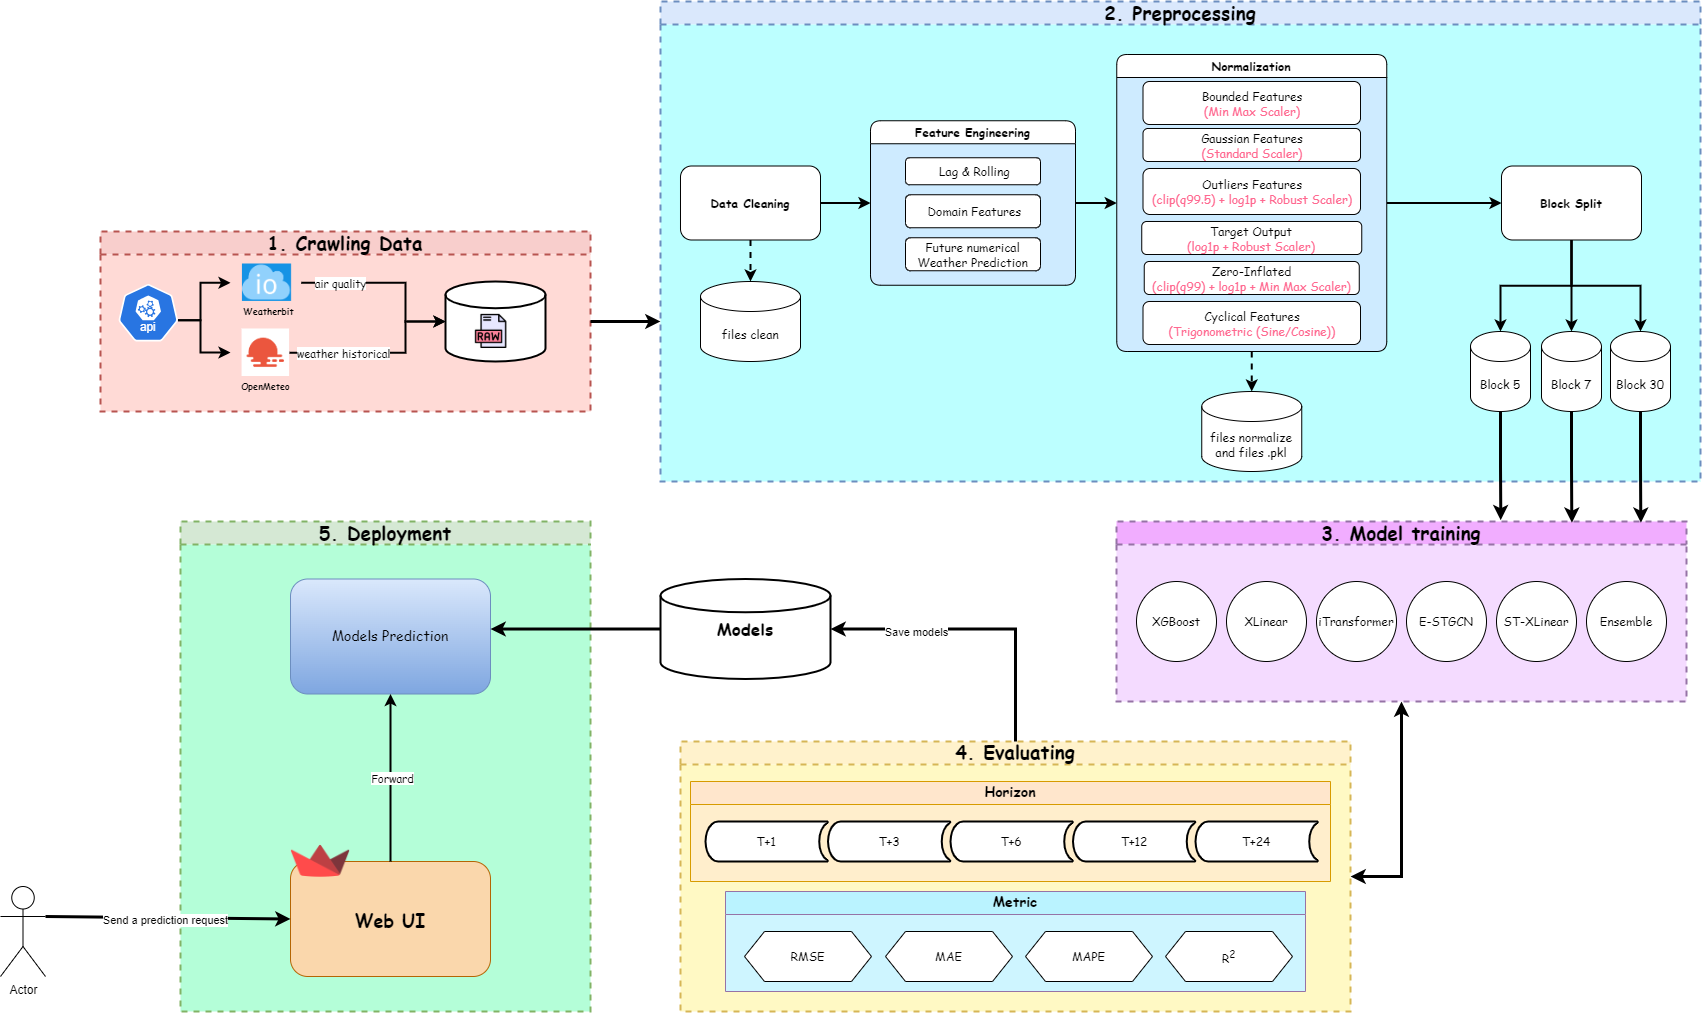
\includegraphics[width=\textwidth]{image/workflow.drawio.png} 
    \caption{Sơ đồ tổng quan giải pháp hệ thống dự báo nồng độ $PM_{2.5}$}
    \label{fig:workflow_tongquan}
\end{figure}

\textbf{Khối 1 --- Thu thập dữ liệu (Crawl Data).} Dữ liệu thô được thu thập tự động từ hai nguồn API: nền tảng Weatherbit cung cấp dữ liệu chất lượng không khí ($PM_{2.5}$, $PM_{10}$, $CO$, $O_3$, $NO_2$, $SO_2$) và nền tảng OpenMeteo cung cấp dữ liệu khí tượng lịch sử (nhiệt độ, độ ẩm, nhiệt độ điểm sương, lượng mưa, mây, tốc độ gió, hướng gió, gió giật, nhiệt độ và độ ẩm đất). Dữ liệu từ 12 trạm quan trắc trong giai đoạn 2023--2025 được lưu trữ dưới dạng tệp thô trước khi đưa vào quy trình xử lý.

\textbf{Khối 2 --- Tiền xử lý dữ liệu (Process).} Dữ liệu thô trải qua bốn giai đoạn xử lý nối tiếp, mỗi giai đoạn tạo ra sản phẩm trung gian phục vụ giai đoạn tiếp theo:

\begin{itemize}
    \item \textit{Data Cleaning:} Thực hiện ghép nối dữ liệu không khí và khí tượng, phát hiện và gắn cờ các bản ghi bất thường (dữ liệu đóng băng, lỗi cảm biến $PM_{2.5}$, giá trị ngoại lai), loại bỏ bản ghi trùng lặp, nội suy giá trị khuyết thiếu, và tạo các đặc trưng phái sinh. Sản phẩm đầu ra là các tệp dữ liệu sạch (files clean).
    
    \item \textit{Feature Engineering:} Tinh chiết các đặc trưng mới dựa trên nguyên lý hóa khí quyển (chỉ số oxidation potential, humid sulfate risk, thermal stability), phân tách thành phần gió ($\sin$/$\cos$), và trích xuất đặc trưng trượt (lag features, rolling mean, rolling std) cùng mã hóa chu kỳ thời gian.
    
    \item \textit{Normalization:} Áp dụng các chiến lược chuẩn hóa khác nhau tùy theo đặc tính phân phối của từng nhóm biến, bao gồm các tổ hợp $Log1p$, $RobustScaler$, $StandardScaler$ và $MinMaxScaler$. Các bộ biến đổi (scalers) được khớp (fit) trên tập huấn luyện và lưu trữ dưới dạng tệp .pkl để phục vụ quá trình giải chuẩn hóa khi suy luận.
    
    \item \textit{Block Split:} Phân chia dữ liệu theo cấu trúc khối thời gian tuần hoàn (cyclic block splitting) với ba cấu hình: Block~5 (chu kỳ 5 ngày: 3 ngày train, 1 ngày val, 1 ngày test), Block~7 (chu kỳ 7 ngày: 5 ngày train, 1 ngày val, 1 ngày test) và Block~30 (chu kỳ 30 ngày: 20 ngày train, 5 ngày val, 5 ngày test). Chiến lược chia theo khối tuần hoàn đảm bảo mỗi tập con đều bao phủ được các điều kiện khí tượng đa dạng qua các mùa, thay vì tập trung vào một giai đoạn thời gian cố định.
\end{itemize}

\textbf{Khối 3 --- Huấn luyện mô hình (Model Train).} Dữ liệu sau phân chia được đưa vào hệ thống đối chuẩn (benchmark) song song giữa sáu kiến trúc mô hình: XGBoost, XLinear, iTransformer, E-STGCN, ST-XLinear (mô hình đề xuất) và Ensemble. Trọng số của các mô hình sau huấn luyện được lưu trữ vào cơ sở dữ liệu mô hình (Models) để phục vụ cả quá trình đánh giá lẫn triển khai.

\textbf{Khối 4 --- Đánh giá hiệu suất (Evaluation).} Kết quả dự báo được đánh giá trên năm tầm nhìn ($T+1$, $T+3$, $T+6$, $T+12$, $T+24$ giờ), sử dụng bốn chỉ số: $RMSE$ \cite{chai2014rmse}, $MAE$ \cite{willmott2005mae}, $MAPE$ \cite{armstrong1992mape} và $R^2$ \cite{nagelkerke1991r2}. Việc đánh giá đa tầm nhìn và đa chỉ số cho phép so sánh hiệu suất của từng kiến trúc trên các kịch bản dự báo ngắn hạn đến dài hạn.

\textbf{Khối 5 --- Triển khai ứng dụng (Deployment).} Mô hình đạt hiệu suất phù hợp được nạp từ cơ sở dữ liệu mô hình vào module suy luận (Model Prediction), sau đó chuyển tiếp kết quả dự báo lên giao diện Web UI xây dựng trên nền tảng Streamlit, cung cấp khả năng giám sát chất lượng không khí và cảnh báo sớm.

Sơ đồ giải pháp trên là khung tham chiếu xuyên suốt cho các chương tiếp theo: \textbf{Chương 2} trình bày chi tiết phương tiện và phương pháp nghiên cứu tương ứng với Khối 1 đến Khối 3, trong khi \textbf{Chương 3} phân tích kết quả thực nghiệm từ Khối 4 và thảo luận về hiệu quả triển khai tại Khối 5.


\section{Phương tiện nghiên cứu}

\subsection{Ngôn ngữ lập trình và thư viện}

Danh sách các công cụ và thư viện chính được sử dụng trong nghiên cứu được tổng hợp tại Bảng \ref{tab:cong_cu_thu_vien}.

\begin{table}[H]
    \centering
    \caption{Danh sách công cụ và thư viện}
    \label{tab:cong_cu_thu_vien}
    \renewcommand{\arraystretch}{1.3}
    \begin{tabular}{p{4cm} p{6.5cm} p{3cm}}
    \toprule
    \textbf{Công cụ} & \textbf{Chức năng} & \textbf{Phiên bản} \\
    \midrule
    Python & Ngôn ngữ lập trình & 3.10+ \\
    Pandas, NumPy & Xử lý dữ liệu bảng, tính toán số học & $\ge$ 2.0 \\
    scikit-learn & KNNImputer, RobustScaler, StandardScaler, MinMaxScaler & $\ge$ 1.3 \\
    XGBoost & Gradient boosting & $\ge$ 2.0 \\
    PyTorch & Deep learning & $\ge$ 2.1 \\
    PyTorch Geometric & Xử lý dữ liệu đồ thị & $\ge$ 2.4 \\
    Streamlit & Ứng dụng web & $\ge$ 1.30 \\
    Matplotlib, Seaborn & Trực quan hóa & --- \\
    \bottomrule
    \end{tabular}
\end{table}

\subsection{Phần cứng}

Toàn bộ quá trình tiền xử lý dữ liệu, huấn luyện mô hình và triển khai ứng dụng được thực hiện trên máy tính xách tay với cấu hình được trình bày tại Bảng \ref{tab:phan_cung}.

\begin{table}[H]
    \centering
    \caption{Cấu hình phần cứng sử dụng trong nghiên cứu}
    \label{tab:phan_cung}
    \renewcommand{\arraystretch}{1.3}
    \begin{tabular}{p{3cm} p{11.3cm}}
    \toprule
    \textbf{Thành phần} & \textbf{Thông số} \\
    \midrule
    CPU & Intel Core i5-12500H (12 nhân, 16 luồng, xung tối đa 4.5 GHz) \\
    RAM & 16 GB DDR5 bus 3200 MHz \\
    GPU & NVIDIA GeForce RTX 3050 Laptop (4 GB GDDR6, nhân CUDA) \\
    \bottomrule
    \end{tabular}
\end{table}

Bộ xử lý i5-12500H với 12 nhân cho phép thực hiện song song các tác vụ tiền xử lý dữ liệu trên $\approx 1{,}63$ triệu bản ghi. RAM 16 GB đảm bảo khả năng nạp toàn bộ ma trận đặc trưng vào bộ nhớ cho các thao tác chuẩn hóa và chia khối. GPU RTX 3050 với 4 GB VRAM được sử dụng để tăng tốc huấn luyện các mô hình học sâu (ESTGCN, ST-XLinear, iTransformer, XLinear) thông qua cơ chế tính toán song song trên nhân CUDA, giúp quá trình lan truyền ngược và tối ưu AdamW hội tụ trong giới hạn thời gian thực tế phục vụ nghiên cứu.
\section{Thu thập dữ liệu}

Dữ liệu đầu vào gồm hai nguồn chính: dữ liệu chất lượng không khí và dữ liệu thời tiết lịch sử, được thu thập song song cho cùng 32 trạm với cùng khoảng thời gian và tần suất.

\subsection{Dữ liệu chất lượng không khí}
Hệ thống thu thập dữ liệu chất lượng không khí được khai thác thông qua dịch vụ nguồn mở Weatherbit API. Nhằm đảm bảo mức độ chi tiết và tính đại diện cho bài toán dự báo chuỗi thời gian, dữ liệu được thu thập liên tục từ ngày 01/01/2023 đến 01/12/2025 tạo thành một chuỗi quan trắc liên tục dài khoảng 25.536 giờ tại mỗi trạm. Với tần suất 1 quan trắc/giờ, mạng lưới trải dài trên 32 trạm phân bố rộng khắp 13 tỉnh/thành phố, đem lại khả năng đối chiếu dữ liệu bề mặt đáng tin cậy. Tổng cộng 7 biến đặc trưng đo lường được sử dụng bao gồm: chỉ số AQI tổng hợp, hai phân loại bụi hạt ($PM_{2.5}$, $PM_{10}$) và khối 4 biến khí hỗn hợp ($CO$, $NO_2$, $SO_2$, $O_3$). Trong đó, nồng độ $PM_{2.5}$ đóng vai trò là biến mục tiêu định hướng cho quá trình hội tụ của toàn bộ hệ thống mô hình dự báo.

\subsection{Dữ liệu thời tiết lịch sử}

Dữ liệu thời tiết lịch sử được thu thập thông qua Open-Meteo API, dựa trên bộ dữ liệu tái phân tích ERA5 của Trung tâm Dự báo Khí tượng Hạn vừa Châu Âu (ECMWF). ERA5 kết hợp dữ liệu quan trắc thực tế từ các trạm khí tượng, vệ tinh và phao biển với mô hình khí tượng số thông qua phương pháp đồng hóa dữ liệu, tạo ra bộ dữ liệu lưới toàn cầu có độ phân giải không gian $0{,}25^\circ \times 0{,}25^\circ$. Độ phân giải này tương đương mỗi ô lưới có kích thước khoảng $28 \times 28$ km tại vĩ độ Việt Nam ($\approx 10$--$21^\circ N$), nghĩa là các giá trị khí tượng đại diện cho trung bình không gian trên một ô vuông cạnh 28 km thay vì giá trị đo tại một điểm duy nhất.

Dữ liệu được thu thập liên tục từ ngày 01/01/2023 đến 01/12/2025, với tần suất 1 bản ghi/giờ, đồng nhất hoàn toàn với nguồn dữ liệu chất lượng không khí. Tổng cộng 17 biến khí tượng thuộc 7 nhóm được thu thập (Bảng \ref{tab:bien_thoi_tiet}).

\begin{table}[H]
    \centering
    \caption{Danh sách 17 biến thời tiết thu thập}
    \label{tab:bien_thoi_tiet}
    \renewcommand{\arraystretch}{1.3}
    \begin{tabular}{p{3cm} p{7cm} p{2.5cm} p{1.5cm}}
    \toprule
    \textbf{Nhóm} & \textbf{Biến} & \textbf{Đơn vị} & \textbf{Số biến} \\
    \midrule
    Nhiệt độ & Nhiệt độ không khí, điểm sương, nhiệt độ cảm nhận & $^\circ$C & 3 \\
    Độ ẩm & Độ ẩm tương đối & \% & 1 \\
    Giáng thủy & Lượng mưa & mm/h & 1 \\
    Mây & Độ phủ mây & \% & 1 \\
    Gió & Tốc độ gió, hướng gió, gió giật & m/s, $^\circ$, m/s & 3 \\
    Nhiệt độ đất & Tại 4 tầng sâu: 0--7, 7--28, 28--100, 100--255 cm & $^\circ$C & 4 \\
    Độ ẩm đất & Tại 4 tầng sâu: 0--7, 7--28, 28--100, 100--255 cm & $m^3/m^3$ & 4 \\
    \bottomrule
    \end{tabular}
\end{table}


Ngoài các yếu tố khí tượng cơ bản ảnh hưởng đến sự phân tán ô nhiễm (nhiệt độ, độ ẩm, tốc độ gió), nhóm nhiệt độ đất và độ ẩm đất (8 biến đo tại 4 tầng sâu từ 0 đến 255 cm) phản ánh điều kiện nhiệt lực học bề mặt --- yếu tố quyết định khả năng đối lưu và chiều cao tầng ranh giới khí quyển, từ đó ảnh hưởng trực tiếp đến nồng độ bụi $PM_{2.5}$ tầng thấp.

\subsection{Siêu dữ liệu}

Tệp siêu dữ liệu chứa tọa độ địa lý (vĩ độ, kinh độ), tỉnh/thành phố và quận/huyện của từng trạm. Thông tin tọa độ được sử dụng để tính khoảng cách Haversine giữa các cặp trạm, từ đó xây dựng ma trận kề cho các mô hình không gian--thời gian (ESTGCN, ST-XLinear). 

Khoảng cách Haversine là đại lượng đo lường khoảng cách vòng lớn ngắn nhất giữa hai điểm trên bề mặt của một hình cầu (trong trường hợp này là Trái Đất), dựa trên tọa độ vĩ độ và kinh độ của chúng. Khác với khoảng cách Euclidean (khoảng cách đường thẳng) vốn giả định bề mặt quan sát là một mặt phẳng, công thức Haversine xét đến độ cong của bề mặt Trái Đất. Đặc tính này mang lại độ chính xác cao hơn đáng kể khi tính toán khoảng cách thực tế giữa các trạm quan trắc địa lý đặt cách xa nhau.

Về mặt toán học, khoảng cách $d$ giữa hai trạm có tọa độ vĩ độ, kinh độ lần lượt là $(\phi_1, \lambda_1)$ và $(\phi_2, \lambda_2)$ (được tính bằng đơn vị radian) được xác định thông qua hệ phương trình:
\begin{equation}
    a = \sin^2\left(\frac{\phi_2 - \phi_1}{2}\right) + \cos(\phi_1)\cos(\phi_2)\sin^2\left(\frac{\lambda_2 - \lambda_1}{2}\right)
\end{equation}
\begin{equation}
    c = 2 \cdot \text{atan2}\left(\sqrt{a}, \sqrt{1-a}\right)
\end{equation}
\begin{equation}
    d = R \cdot c
\end{equation}
trong đó, $R \approx 6371 \text{ km}$ là bán kính trung bình của Trái Đất. Giá trị $d$ thu được chính là nền tảng để thiết lập cường độ liên kết không gian ban đầu giữa các nút mạng trong đồ thị. Tổng quy mô dữ liệu thô đạt khoảng 1,63 triệu bản ghi (32 trạm $\times$ 25.536 giờ $\times$ 2 nguồn), tạo nền tảng bao quát cho mạng cảm biến đa trạm.\section{Khảo sát và chọn lọc trạm quan trắc}

\subsection{Sự cần thiết của bước chọn lọc}

Trong 32 trạm ban đầu, không phải trạm nào cũng đáp ứng yêu cầu về chất lượng dữ liệu và tính đại diện vùng. Các vấn đề quan sát được bao gồm: tỷ lệ dữ liệu khuyết cao (một số trạm > 40\%), cảm biến hỏng gây dữ liệu đóng băng, dữ liệu trùng lặp giữa các trạm cùng khu vực ($r > 0.99$), hoặc trạm cô lập không có trạm lân cận để mô hình spatio-temporal khai thác.

\subsection{Hệ thống tiêu chí lọc}

Sáu tiêu chí được thiết kế và đánh giá tuần tự trên 32 trạm.

\begin{table}[H]
    \centering
    \caption{Hệ thống 6 tiêu chí lọc}
    \label{tab:he_thong_tieu_chi}
    \renewcommand{\arraystretch}{1.3}
    \begin{tabular}{p{1.5cm} p{3cm} p{4.5cm} p{5cm}}
    \toprule
    \textbf{Ký hiệu} & \textbf{Tiêu chí} & \textbf{Ngưỡng} & \textbf{Phương pháp đánh giá} \\
    \midrule
    R1 & Data Integrity & Missing $PM_{2.5} < 20\%$ & Đếm số giờ NaN / tổng số giờ kỳ vọng \\
    R2 & Frozen Sensor & Frozen events < 50 & Đếm số đoạn có rolling std < $10^{-6}$ trên cửa sổ 12h \\
    R3 & Spatial Clustering & $\ge 1$ trạm khác trong bán kính 100 km & Tính khoảng cách Haversine giữa tất cả các cặp trạm \\
    R4 & Data Uniqueness & Hệ số tương quan Pearson $r < 0.99$ & Tính $r$ giữa chuỗi $PM_{2.5}$ của các cặp trạm cùng cụm \\
    R5 & Climate Homogeneity & Cùng vùng khí hậu trong cụm & Phân loại theo ranh giới địa lý Bắc/Nam \\
    R6 & Variance & Cụm có đa dạng loại trạm & Kiểm tra phân bố: đô thị / ngoại ô / ven biển \\
    \bottomrule
    \end{tabular}
\end{table}


Hệ thống tiêu chí này được chia thành ba nhóm cấp độ đánh giá chặt chẽ. Cụ thể, các tiêu chí R1--R2 nhằm bảo đảm tính toàn vẹn và giới hạn lỗi đóng băng dữ liệu nội tại ở từng trạm đơn lẻ. Nhóm R3--R4 kiểm soát các mối quan hệ không gian, loại bỏ khu vực cô lập với hệ số $r$ trùng lặp vượt ngưỡng, tối ưu hóa biểu diễn học không gian. Cuối cùng, nhóm R5--R6 phân tách khí hậu và phương diện địa giới, bảo chứng cho sự đa dạng đặc trưng của từng cụm khu vực nghiên cứu.


\subsection{Kết quả chọn lọc}

Sau khi áp dụng 6 tiêu chí, 12/32 trạm (37.5\%) vượt qua toàn bộ và được chia thành 2 cụm vùng (Bảng \ref{tab:12_tram_duoc_chon}).

\begin{table}[H]
    \centering
    \caption{12 trạm được chọn, phân theo cụm vùng}
    \label{tab:12_tram_duoc_chon}
    \renewcommand{\arraystretch}{1.3}
    \begin{tabular}{p{4cm} p{1.5cm} p{8.5cm}}
    \toprule
    \textbf{Cụm} & \textbf{ID} & \textbf{Tỉnh/Thành --- Quận/Huyện} \\
    \midrule
    \textbf{Bắc (North)} & 1 & Hà Nội --- Cầu Giấy \\
    & 4 & Thanh Hóa --- Thọ Xuân \\
    & 5 & Hà Nội --- Gia Lâm \\
    & 16 & Hải Phòng --- Đồ Sơn \\
    & 17 & Hải Phòng --- Hồng Bàng \\
    & 27 & Nam Định --- TP. Nam Định \\
    \midrule
    \textbf{Nam (South)} & 7 & TP. HCM --- Quận 1 \\
    & 18 & Cần Thơ --- Ninh Kiều \\
    & 24 & Đồng Nai --- Biên Hòa \\
    & 30 & Vĩnh Long --- TP. Vĩnh Long \\
    & 31 & Trà Vinh --- TP. Trà Vinh \\
    & 32 & An Giang --- Rạch Giá \\
    \bottomrule
    \end{tabular}
\end{table}

\begin{figure}[H]
    \centering
    
    % Miền Bắc
    \begin{subfigure}{0.48\textwidth}
        \centering
        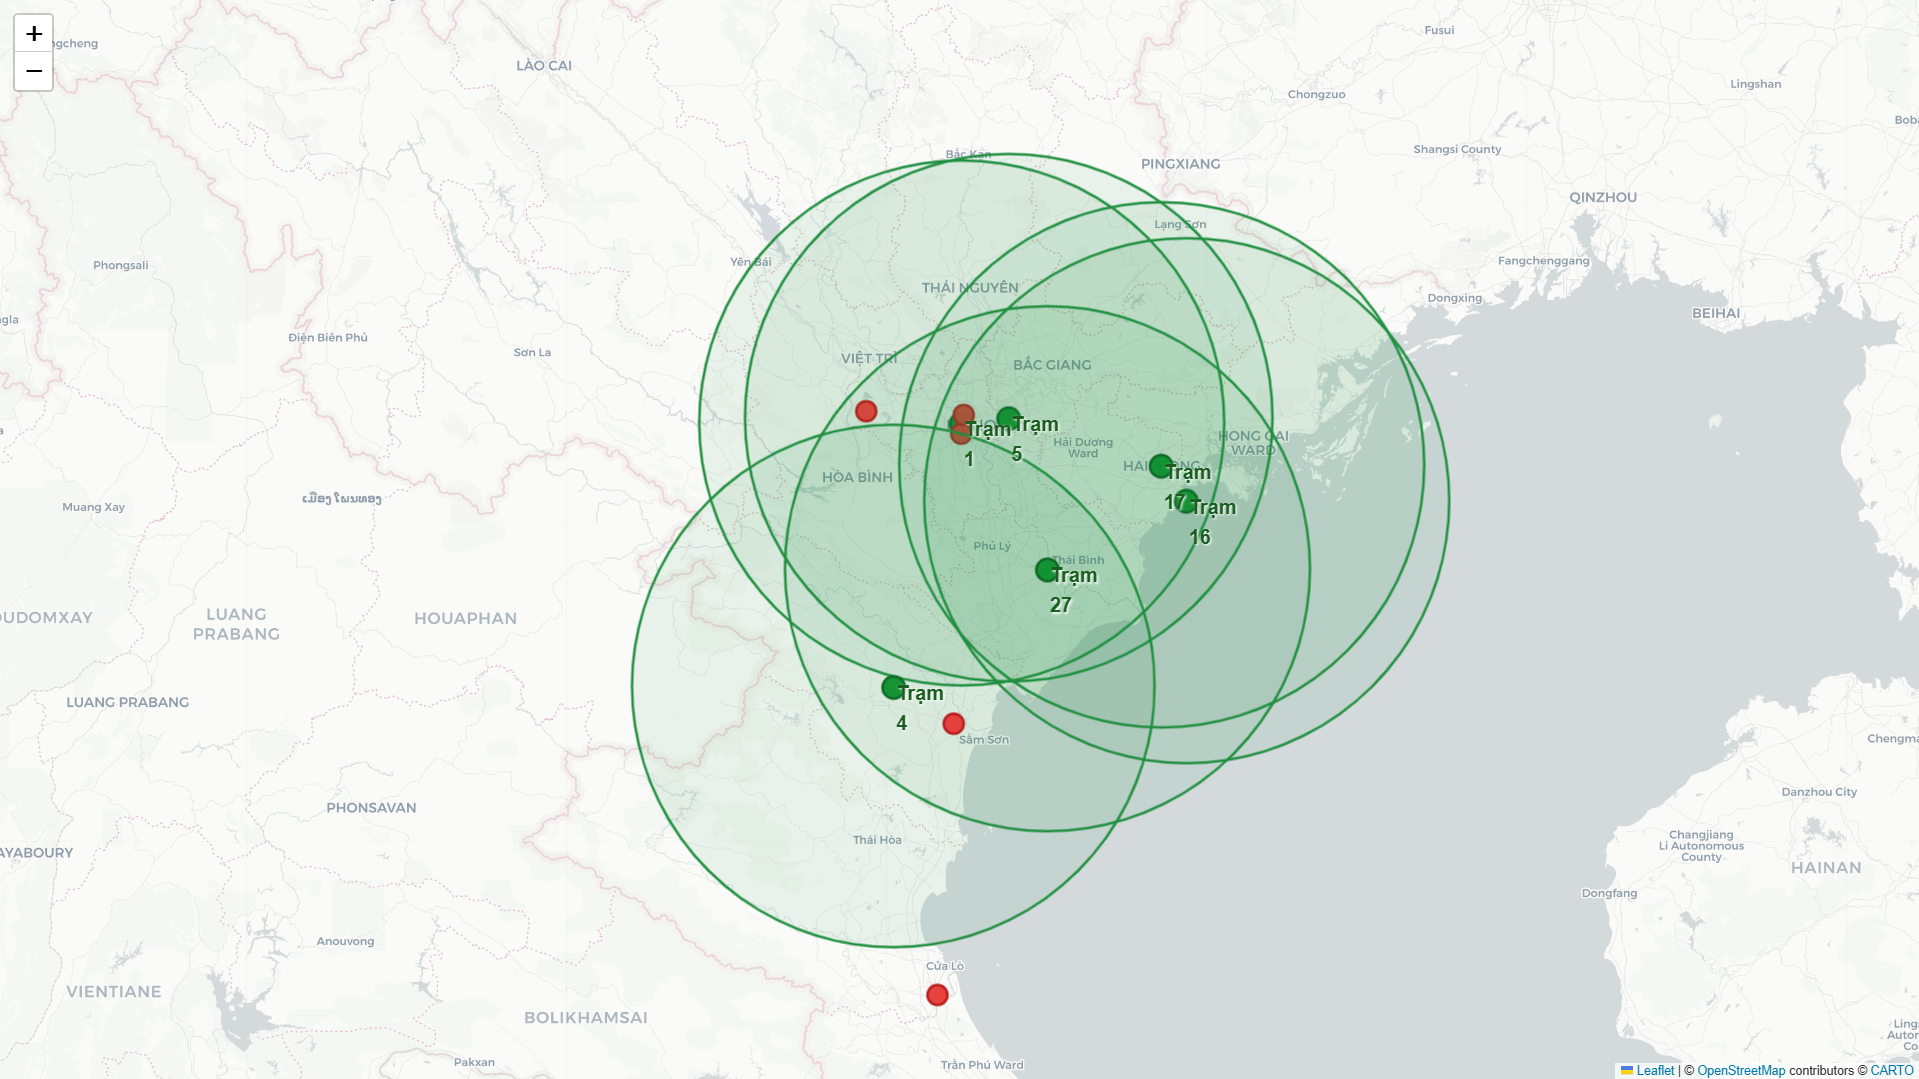
\includegraphics[width=\linewidth]{image/cluster_north.png}
        \caption{Cụm trạm khu vực miền Bắc}
        \label{fig:cluster_north}
    \end{subfigure}
    \hfill
    % Miền Nam
    \begin{subfigure}{0.48\textwidth}
        \centering
        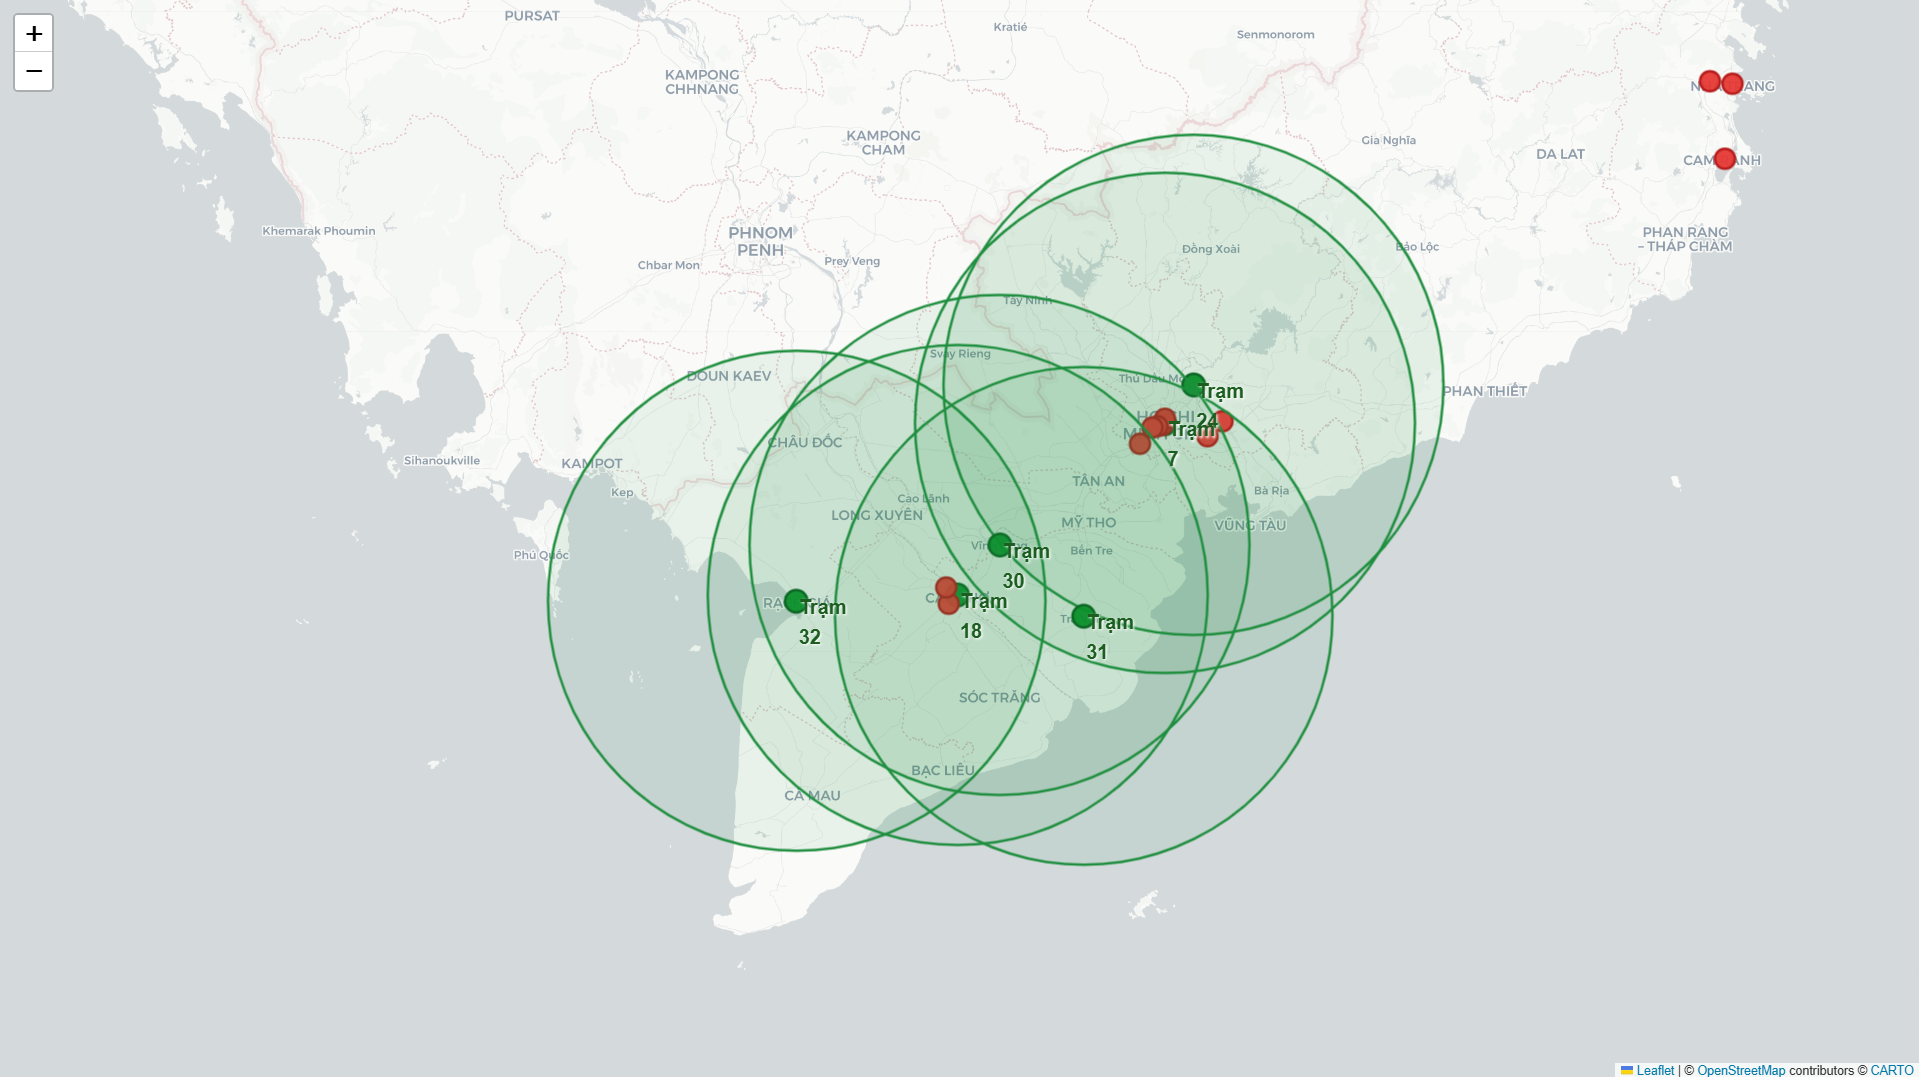
\includegraphics[width=\linewidth]{image/cluster_south.png}
        \caption{Cụm trạm khu vực miền Nam}
        \label{fig:cluster_south}
    \end{subfigure}

    \caption{Phân bố các trạm quan trắc theo hai cụm miền Bắc và miền Nam}
    \caption*{Các vòng tròn màu xanh biểu diễn bán kính lân cận của từng trạm. 
    Điểm màu xanh là trạm được chọn, điểm màu đỏ là các vị trí lân cận.}
    
    \label{fig:ban_do_12_tram}
\end{figure}

Việc phân 2 cụm Bắc/Nam dựa trên đặc tính phân phối $PM_{2.5}$: cụm Bắc có biên độ $PM_{2.5}$ theo mùa lớn (trung bình mùa đông gấp 2--3 lần mùa hè), trong khi cụm Nam có nồng độ $PM_{2.5}$ ổn định hơn quanh năm. Do sự khác biệt phân phối này, mỗi cụm được huấn luyện mô hình dự báo riêng biệt.

\section{Tiền xử lý dữ liệu --- Làm sạch}

Quy trình làm sạch dữ liệu được thực hiện độc lập cho mỗi trạm quan trắc, bao gồm 7 bước tuần tự chia thành 3 giai đoạn chính (Hình \ref{fig:pipeline_clean}):

Quy trình tiền xử lý dữ liệu được tiến hành tuần tự qua ba giai đoạn có mối liên hệ chặt chẽ với nhau. Khởi đầu với \textbf{giai đoạn ghép nối và chuẩn bị} (Bước 1--2), hai nguồn dữ liệu độc lập về chất lượng không khí và khí tượng tại mỗi trạm được đồng bộ hóa dựa trên nhãn thời gian. Ngay sau đó, biến hướng gió được mã hóa tuần hoàn và một chỉ mục giờ liên tục được thiết lập nhằm định vị chính xác các khoảng dữ liệu bị khuyết. Dựa trên nền tảng này, hệ thống chuyển sang \textbf{giai đoạn phát hiện và gán nhãn lỗi} (Bước 3--5) bằng cách quét tuần tự toàn bộ chuỗi để nhận diện ba nhóm dị thường chính: hiện tượng đóng băng cảm biến, các giá trị ngoại lai và lỗi xuất phát từ cảm biến quang học. Những điểm dữ liệu vi phạm sẽ được hệ thống tự động gán nhãn cảnh báo hoặc loại bỏ. Cuối cùng, tại \textbf{giai đoạn làm sạch và phục hồi} (Bước 6--7), các bản ghi trùng lặp được tinh giản hoàn toàn. Những khoảng trống dữ liệu để lại sẽ được khôi phục linh hoạt: phương pháp nội suy tuyến tính được áp dụng cho các gián đoạn ngắn, trong khi thuật toán K-láng giềng gần nhất (KNN) được sử dụng để xử lý các khoảng mất mát lớn. Kết thúc quy trình, tập dữ liệu thô đã được chuyển hóa thành một chuỗi thời gian liên tục, toàn vẹn và sẵn sàng cho bước kỹ nghệ đặc trưng tiếp theo.

\begin{figure}[H]
    \centering
    \begin{tikzpicture}[
        node distance=1.2cm,
        % Đầu vào / Đầu ra
        io/.style={
            rectangle, draw=black!50, fill=gray!10,
            text width=14em, text centered, rounded corners,
            minimum height=2.5em, font=\small\itshape
        },
        % Tiêu đề giai đoạn 1
        phaseA/.style={
            rectangle, draw=blue!60, fill=blue!15,
            text width=14em, text centered, rounded corners,
            minimum height=2.5em, font=\small\bfseries
        },
        % Bước thuộc giai đoạn 1
        stepA/.style={
            rectangle, draw=blue!40, fill=blue!5,
            text width=13em, text centered, rounded corners,
            minimum height=2.5em, font=\small
        },
        % Tiêu đề giai đoạn 2
        phaseB/.style={
            rectangle, draw=orange!60, fill=orange!15,
            text width=14em, text centered, rounded corners,
            minimum height=2.5em, font=\small\bfseries
        },
        % Bước thuộc giai đoạn 2
        stepB/.style={
            rectangle, draw=orange!40, fill=orange!5,
            text width=13em, text centered, rounded corners,
            minimum height=2.5em, font=\small
        },
        % Tiêu đề giai đoạn 3
        phaseC/.style={
            rectangle, draw=teal!60, fill=teal!15,
            text width=14em, text centered, rounded corners,
            minimum height=2.5em, font=\small\bfseries
        },
        % Bước thuộc giai đoạn 3
        stepC/.style={
            rectangle, draw=teal!40, fill=teal!5,
            text width=13em, text centered, rounded corners,
            minimum height=2.5em, font=\small
        },
        % Mũi tên
        arr/.style={-latex, thick, draw=gray!60}
    ]
        % Đầu vào
        \node [io] (input) {Dữ liệu thô (không khí + thời tiết)};

        % Giai đoạn 1
        \node [phaseA, below of=input] (p1) {Giai đoạn 1: Ghép nối và chuẩn bị};
        \node [stepA, below of=p1] (s1) {Bước 1: Phân tách thành phần gió};
        \node [stepA, below of=s1] (s2) {Bước 2: Kiểm tra khoảng thời gian};

        % Giai đoạn 2
        \node [phaseB, below of=s2] (p2) {Giai đoạn 2: Phát hiện và gán nhãn lỗi};
        \node [stepB, below of=p2] (s3) {Bước 3: Phát hiện dữ liệu đóng băng};
        \node [stepB, below of=s3] (s4) {Bước 4: Phát hiện ngoại lai};
        \node [stepB, below of=s4] (s5) {Bước 5: Phát hiện lỗi cảm biến quang học};

        % Giai đoạn 3
        \node [phaseC, below of=s5] (p3) {Giai đoạn 3: Làm sạch và phục hồi};
        \node [stepC, below of=p3] (s6) {Bước 6: Xóa trùng lặp};
        \node [stepC, below of=s6] (s7) {Bước 7: Điền giá trị khuyết};

        % Đầu ra
        \node [io, below of=s7] (output) {Chuỗi thời gian liên tục};

        % Mũi tên nối
        \draw [arr] (input) -- (p1);
        \draw [arr] (p1) -- (s1);
        \draw [arr] (s1) -- (s2);
        \draw [arr] (s2) -- (p2);
        \draw [arr] (p2) -- (s3);
        \draw [arr] (s3) -- (s4);
        \draw [arr] (s4) -- (s5);
        \draw [arr] (s5) -- (p3);
        \draw [arr] (p3) -- (s6);
        \draw [arr] (s6) -- (s7);
        \draw [arr] (s7) -- (output);

    \end{tikzpicture}
    \caption{Quy trình làm sạch dữ liệu cho mỗi trạm quan trắc}
    \caption*{Quy trình gồm 3 giai đoạn và 7 bước tuần tự. Đầu vào là dữ liệu thô đã ghép nối, đầu ra là chuỗi thời gian liên tục sẵn sàng cho bước kỹ thuật đặc trưng.}
    \label{fig:pipeline_clean}
\end{figure}

\subsection{Bước 1 --- Mã hóa tuần hoàn và phân tách thành phần gió}

Trong dữ liệu khí tượng, hướng gió (đơn vị độ) là một biến đặc trưng mang tính tuần hoàn cao, nơi các giá trị $0^\circ$ và $360^\circ$ cùng biểu diễn một thực thể vật lý duy nhất là hướng Bắc. Tuy nhiên, sự chênh lệch số học cực đại giữa hai giá trị này ($|360 - 0| = 360$) tạo ra một điểm gãy nghiêm trọng trong không gian đặc trưng. Hiện tượng này khiến các mô hình học máy và mạng nơ-ron dễ hiểu lầm rằng gió hướng $1^\circ$ và $359^\circ$ là hai trạng thái đối lập về mặt địa lý, trong khi thực tế chúng gần như trùng khít. Để khắc phục triệt để sự gián đoạn này, hướng gió gốc $\theta$ cần được chuyển đổi sang đơn vị radian và mã hóa vào không gian hai chiều thông qua các hàm lượng giác sin và cosin theo các công thức sau:

\begin{equation}
    W_{sin} = \sin\left(\theta \times \frac{\pi}{180}\right)
\end{equation}
\begin{equation}
    W_{cos} = \cos\left(\theta \times \frac{\pi}{180}\right)
\end{equation}

Việc phân tách này không chỉ đơn thuần là thay đổi đơn vị đo lường mà còn mang ý nghĩa vật lý quan trọng trong phân tích động lực học khí quyển. Thành phần $W_{sin}$ đại diện cho vector gió dọc theo trục Đông -- Tây (nhận giá trị dương khi gió thổi từ phía Đông và âm khi từ phía Tây), trong khi $W_{cos}$ đại diện cho trục Bắc -- Nam (nhận giá trị dương khi gió từ phía Bắc và âm khi từ phía Nam). Kết quả là hướng gió được biểu diễn bởi một cặp giá trị biến thiên liên tục trong khoảng $[-1, 1]$, tạo thành một vector đơn vị trên vòng tròn lượng giác. Cách tiếp cận này giúp loại bỏ hoàn toàn sự nhảy vọt về giá trị tại điểm chuyển giao $0^\circ/360^\circ$, hỗ trợ mô hình học sâu nắm bắt được các tương quan không gian một cách chính xác và ổn định hơn. Sau khi quá trình mã hóa hoàn tất, biến hướng gió gốc sẽ được loại bỏ để tối ưu hóa không gian đầu vào và tránh gây nhiễu cho quá trình huấn luyện.\subsection{Bước 2 --- Kiểm tra khoảng thời gian}

Hệ thống tạo chỉ mục giờ đầy đủ từ 00:00 ngày 01/01/2023 đến 23:00 ngày 01/12/2025 (tổng cộng 25.536 mốc giờ kỳ vọng cho mỗi trạm). Dữ liệu gốc được gán vào chỉ mục này; các mốc giờ thiếu dữ liệu sẽ tự động nhận giá trị rỗng. Bước này giúp xác định chính xác tỷ lệ dữ liệu khuyết theo công thức: $(\text{số giờ rỗng} / \text{tổng số giờ kỳ vọng}) \times 100\%$.

\subsection{Bước 3 --- Phát hiện dữ liệu đóng băng}

Hiện tượng đóng băng xảy ra khi cảm biến gặp sự cố phần cứng hoặc mất kết nối, khiến giá trị đầu ra không thay đổi trong nhiều giờ liên tiếp. Mục tiêu của bước này là phát hiện và gán nhãn các khung giờ đóng băng để mô hình nhận biết dữ liệu không đáng tin cậy.

Phương pháp phát hiện thực hiện tính độ lệch chuẩn trượt trên cửa sổ 12 giờ (yêu cầu tối thiểu 6 quan sát hợp lệ, lấy tâm giữa cửa sổ) cho toàn bộ 11 biến quan trắc chủ chốt. Cụ thể, các biến này bao gồm 7 biến ô nhiễm ($AQI$, $PM_{2.5}$, $PM_{10}$, $CO$, $NO_2$, $SO_2$, $O_3$) và 4 biến khí tượng đi kèm (nhiệt độ, độ ẩm tương đối, điểm sương, tốc độ gió). Nếu độ lệch chuẩn tại một mốc thời gian bất kỳ có giá trị $< 10^{-6}$ (tức gần như không biến thiên), khung giờ đó được gán nhãn đóng băng. Cửa sổ 12 giờ được lựa chọn vì đủ dài để phát hiện tình trạng đóng băng xuyên đêm, và phép lấy tâm giữa cửa sổ cho phép nhận diện chính xác các rìa biên của đoạn lỗi.


\subsection{Bước 4 --- Phát hiện ngoại lai}

Dữ liệu chất lượng không khí thu thập từ các trạm quan trắc có thể chứa các giá trị bất thường do lỗi thiết bị, nhiễu truyền dẫn hoặc các sự kiện phát thải cực đoan. Mục tiêu của bước này là xác định và gán nhãn các giá trị ngoại lai để tách biệt khỏi dữ liệu hợp lệ, tránh ảnh hưởng đến quá trình huấn luyện mô hình. Ngoại lai được phát hiện qua hai tầng bổ trợ.

\textbf{Tầng 1 --- Ngưỡng vật lý:} Mỗi biến được áp dụng khoảng giá trị hợp lệ dựa trên các quy chuẩn kỹ thuật (Bảng \ref{tab:nguong_vat_ly}). Các giá trị nằm ngoài khoảng hợp lệ sẽ được gán nhãn ngoại lai.

\begin{table}[H]
    \centering
    \caption{Ngưỡng vật lý phát hiện ngoại lai}
    \label{tab:nguong_vat_ly}
    \renewcommand{\arraystretch}{1.3}
    \begin{tabular}{p{2.5cm} p{1.5cm} p{1.5cm} p{2.5cm} p{5.5cm}}
    \toprule
    \textbf{Biến} & \textbf{Min} & \textbf{Max} & \textbf{Đơn vị} & \textbf{Nguồn tham chiếu} \\
    \midrule
    AQI & 0 & 500 & --- & \cite{USEPA_AQI} \\
    $PM_{2.5}$ & 0 & 600 & $\mu g/m^3$ & \cite{USEPA_AQI} \\
    $PM_{10}$ & 0 & 1.000 & $\mu g/m^3$ & \cite{QCVN05_2023} \\
    $CO$ & 0 & 20.000 & $\mu g/m^3$ & \cite{QCVN05_2023} \\
    $NO_2$ & 0 & 400 & $\mu g/m^3$ & \cite{QCVN05_2023} \\
    $SO_2$ & 0 & 500 & $\mu g/m^3$ & \cite{QCVN06_2009} \\
    $O_3$ & 0 & 350 & $\mu g/m^3$ & Quan trắc thực tế \\
    Nhiệt độ & 0 & 50 & $^\circ$C & Biên khí hậu Việt Nam \\
    Độ ẩm & 0 & 100 & \% & Giới hạn vật lý \\
    Tốc độ gió & 0 & 20 & m/s & Giá trị theo giờ \\
    \bottomrule
    \end{tabular}
\end{table}


Ngưỡng tối đa cho các chất ô nhiễm được xác định dựa trên Quy chuẩn kỹ thuật quốc gia QCVN 05:2023/BTNMT \cite{QCVN05_2023} và QCVN 06:2009/BTNMT \cite{QCVN06_2009}. Riêng chỉ số AQI và ngưỡng $PM_{2.5}$ áp dụng theo thang đo của Cơ quan Bảo vệ Môi trường Hoa Kỳ \cite{USEPA_AQI}, trong đó mức 600 $\mu g/m^3$ tương ứng với ngưỡng nguy hại cao nhất. Đối với các biến khí tượng, giới hạn được thiết lập theo biên khí hậu đặc trưng của Việt Nam.

\textbf{Tầng 2 --- Khoảng tứ phân vị:} Áp dụng bổ sung cho 6 biến ô nhiễm với hệ số $3 \times IQR$ nhằm bảo toàn các giá trị tăng vọt thực tế (ví dụ: bụi mịn mùa đông tại Hà Nội) \cite{tukey1977eda}. Giá trị $x$ được coi là ngoại lai nếu:
\begin{equation}
    x < Q_1 - 3 \times IQR \quad \text{hoặc} \quad x > Q_3 + 3 \times IQR
\end{equation}

\subsection{Bước 5 --- Phát hiện lỗi cảm biến quang học}

Cảm biến đếm hạt quang học (OPC) có thể phát sinh lỗi phần cứng khiến giá trị đo bụi $PM_{2.5}$ và $PM_{10}$ tăng đột biến mà không phản ánh điều kiện ô nhiễm thực tế. Mục tiêu của bước này là phân biệt giữa đợt tăng nồng độ thực và lỗi thiết bị, từ đó loại bỏ các điểm dữ liệu sai lệch.

Phương pháp phát hiện yêu cầu ba điều kiện phải đồng thời thỏa mãn. Thứ nhất, nồng độ $PM_{2.5}$ vượt quá ngưỡng $Q_3 + 3 \times IQR$ (với IQR được tính trượt theo tháng để loại trừ ảnh hưởng mùa vụ). Thứ hai, nồng độ $PM_{10}$ cũng đồng thời vượt ngưỡng $Q_3 + 3 \times IQR$, xác nhận lỗi xuất phát từ buồng đo chung. Thứ ba, tỷ lệ biến đổi tuyệt đối theo giờ của các chất khí ($CO$, $NO_2$, $SO_2$) phải duy trì dưới 50\%, chứng tỏ không có đợt phát thải thực tế nào đang xảy ra. Chỉ khi cả ba điều kiện đều được kích hoạt, giá trị $PM_{2.5}$ và $PM_{10}$ tại mốc thời gian đó mới bị loại bỏ và chuyển sang bước điền khuyết.

\subsection{Bước 6 --- Xóa trùng lặp}

Quá trình thu thập dữ liệu liên tục từ các API công cộng có thể phát sinh hiện tượng trùng lặp nhãn thời gian do chồng lấn giữa các phiên thu thập hoặc cơ chế thử lại của máy chủ nguồn. Mục tiêu của bước này là đảm bảo mỗi mốc thời gian chỉ xuất hiện duy nhất một lần trong chuỗi dữ liệu.

Hệ thống quét toàn bộ chỉ mục thời gian và loại bỏ mọi bản ghi trùng lặp, chỉ giữ lại bản ghi đầu tiên theo thứ tự xuất hiện. Chiến lược ưu tiên bản ghi đầu dựa trên cơ sở: phiên thu thập sớm nhất thường phản ánh dữ liệu gần nhất với thời điểm quan trắc thực tế. Bước này ngăn ngừa nguy cơ cùng một điểm dữ liệu bị đếm nhiều lần trong quá trình xây dựng cửa sổ trượt và tính toán thống kê ở các giai đoạn sau.

\subsection{Bước 7 --- Điền giá trị khuyết}

Sau khi hoàn tất các bước phát hiện lỗi (đóng băng, ngoại lai, lỗi cảm biến) và xóa trùng lặp, chuỗi dữ liệu chứa các khoảng trống cần được điền khuyết trước khi đưa vào mô hình. Quy trình điền khuyết được thực hiện qua 3 bước tuần tự.

Để khôi phục tính liên tục của chuỗi thời gian, hệ thống áp dụng một chiến lược điền khuyết lai linh hoạt tùy thuộc vào quy mô của khoảng gián đoạn. Đối với các khoảng trống ngắn hạn (nhỏ hơn hoặc bằng 6 giờ liên tiếp), phương pháp nội suy tuyến tính theo trục thời gian được ưu tiên sử dụng, dựa trên đặc tính biến thiên trơn tru và không đột ngột của các yếu tố khí tượng trong quy mô vài giờ. Ngược lại, với các khoảng khuyết dữ liệu lớn (trên 6 giờ), hệ thống chuyển sang sử dụng thuật toán K-láng giềng gần nhất (KNN Imputation) \cite{troyanskaya2001knn} nhằm khai thác tối đa tương quan đa biến. Một bước tiền xử lý mang tính quyết định trước khi chạy KNN là toàn bộ các biến phải được chuẩn hóa tạm thời về cùng một thang đo. Thao tác này ngăn chặn rủi ro các biến có dải giá trị tuyệt đối lớn lấn át các biến có dải giá trị nhỏ trong phép tính toán khoảng cách Euclidean. Thuật toán KNN sau đó được thiết lập với $K=12$ (tương đương nửa chu kỳ ngày đêm của khí quyển) kết hợp cùng trọng số nghịch đảo khoảng cách, giúp các mẫu dữ liệu càng gần gũi về mặt cấu trúc sẽ càng đóng góp lớn vào giá trị ước lượng. Cuối cùng, tại bước hậu xử lý, toàn bộ dữ liệu khuyết sau khi điền được giải chuẩn hóa  về lại đơn vị đo lường gốc, đồng thời các giá trị âm (nếu vô tình phát sinh từ biên giới của phép nội suy) được giới hạn cứng về mức $0$ nhằm bảo toàn nghiêm ngặt ý nghĩa vật lý thực tế của nồng độ chất ô nhiễm.
\section{Kỹ thuật đặc trưng}

\subsection{Tổng quan và lý do thực hiện}

Các biến thô thu thập từ trạm quan trắc chỉ phản ánh giá trị tức thời tại mỗi mốc thời gian, chưa chứa thông tin về xu hướng lịch sử, mức biến động và các mối tương tác giữa các biến. Các nghiên cứu về dự báo chuỗi thời gian chỉ ra rằng hiệu năng mô hình phụ thuộc đáng kể vào chất lượng đặc trưng đầu vào \cite{Chen_2016}. Vì vậy, bước kỹ thuật đặc trưng là cần thiết để:

Quá trình kỹ nghệ đặc trưng đóng vai trò cốt lõi trong việc nâng cao khả năng học biểu diễn của mô hình thông qua nhiều khía cạnh phân tích. Trước hết, việc áp dụng phép trễ cung cấp ngữ cảnh lịch sử quan trọng tại các mốc thời gian trước đó ($t-1, t-3, \ldots, t-24$ giờ), cho phép hệ thống tự động nắm bắt được quy luật quán tính tự nhiên của chuỗi. Bên cạnh đó, các phép thống kê trượt như trung bình, độ lệch chuẩn và giá trị cực đại trên các cửa sổ 12--24 giờ cung cấp thước đo định lượng về xu hướng nền và mức độ biến động gần đây của nồng độ $PM_{2.5}$. Hơn nữa, do nồng độ bụi mịn chịu sự chi phối phức tạp từ nhiều yếu tố đan xen, các đặc trưng tương tác được xây dựng nhằm biểu diễn những hiệu ứng phi tuyến kết hợp giữa nguồn phát thải, điều kiện khí tượng và phản ứng hóa học mà từng biến đơn lẻ không thể lột tả trọn vẹn. Cuối cùng, để củng cố khả năng nhận diện quy luật thời gian, hệ thống tiến hành mã hóa tuần hoàn bằng các hàm lượng giác, qua đó tích hợp liền mạch các tín hiệu chu kỳ mang tính quy luật như lưu lượng giao thông theo giờ, hoạt động sản xuất theo tuần và biến động khí hậu theo mùa.
Từ 24 biến thô ban đầu (7 biến ô nhiễm và 17 biến thời tiết), hệ thống tạo ra tổng cộng 134 đặc trưng phân thành 8 nhóm chính (Bảng \ref{tab:8_nhom_dac_trung}).

\begin{table}[H]
    \centering
    \caption{8 nhóm đặc trưng trong hệ thống}
    \label{tab:8_nhom_dac_trung}
    \renewcommand{\arraystretch}{1.3}
    \begin{tabular}{p{1.5cm} p{8.5cm} p{3cm}}
    \toprule
    \textbf{Nhóm} & \textbf{Tên nhóm} & \textbf{Số lượng} \\
    \midrule
    1 & Đặc trưng thô & 16 \\
    2 & Đặc trưng tương tác & 16 \\
    3 & Cờ chất lượng dữ liệu & 5 \\
    4 & Trễ $PM_{2.5}$ & 7 \\
    5 & Thống kê trượt $PM_{2.5}$ & 6 \\
    6 & Trễ ô nhiễm và thời tiết & 31 \\
    7 & Mã hóa thời gian & 14 \\
    8 & Thời tiết tương lai & $\approx$ 20 \\
    \midrule
    & \textbf{Tổng cộng} & \textbf{$\approx$ 134} \\
    \bottomrule
    \end{tabular}
\end{table}


Nhóm 1--2 mã hóa trạng thái quan trắc hiện tại và các mối tương tác vật lý--hóa học phi tuyến. Nhóm 3 cung cấp nhãn chất lượng dữ liệu. Nhóm 4--6 khai thác thông tin lịch sử thông qua phép trễ và thống kê trượt trên chuỗi thời gian, trong đó tất cả đều được dịch chuyển 1 bước thời gian nhằm ngăn chặn rò rỉ dữ liệu. Nhóm 7 mã hóa chu kỳ tuần hoàn theo giờ, ngày và năm bằng hàm lượng giác $\sin/\cos$. Nhóm 8 bổ sung thông tin thời tiết tại thời điểm tương lai (dịch chuyển theo tầm nhìn dự báo), được thiết kế để tích hợp với nguồn dữ liệu dự báo khí tượng số (NWP) khi triển khai thực tế.

\subsection{Đặc trưng tương tác}

Các đặc trưng tương tác được thiết kế để nắm bắt các mối quan hệ phi tuyến và các chỉ số vật lý/hóa học ảnh hưởng đến nồng độ bụi mịn (Bảng \ref{tab:dac_trung_tuong_tac}).

\begin{table}[H]
    \centering
    \caption{Danh sách các đặc trưng tương tác}
    \label{tab:dac_trung_tuong_tac}
    \renewcommand{\arraystretch}{1.3}
    \begin{tabular}{p{3cm} p{3.5cm} p{4cm} p{3.5cm}}
    \toprule
    \textbf{Đặc trưng} & \textbf{Công thức} & \textbf{Ý nghĩa} & \textbf{Cơ sở} \\
    \midrule
    Tiềm năng oxy hóa & $O_3 \times (SO_2 + NO_2)$ & Chỉ số oxy hóa thứ cấp & Khả năng oxy hóa khí quyển thúc đẩy chuyển hóa tiền chất thành bụi thứ cấp \\
    Tổng tải ô nhiễm & $CO + SO_2 + NO_2$ & Tổng nồng độ các chất từ quá trình đốt cháy & Đặc trưng cho lượng phát thải sơ cấp từ nguồn đốt nhiên liệu hóa thạch \\
    Chỉ số nguồn phát & $\log(NO_2+1) - \log(SO_2+1)$ & Dương: giao thông; Âm: công nghiệp & Tỷ lệ log giữa hai nguồn phát chính \\
    Nguy cơ sulfate ẩm & $\text{độ ẩm} \times SO_2$ & Chỉ số hình thành aerosol sulfate & Phản ứng oxy hóa pha lỏng chuyển hóa $SO_2$ thành sulfate ($SO_4^{2-}$) khi ẩm cao \\
    Ổn định nhiệt & $T_{air} - T_{soil\_0}$ & Dương: đối lưu; Âm: nghịch nhiệt & Chênh lệch nhiệt bề mặt--khí quyển \\
    Tiềm năng cuốn bụi & $v_{wind} / (\theta_{soil} + 1)$ & Chỉ số cuốn bụi cơ học & Tỷ lệ lực gió trên sức kết dính đất \\
    Chỉ số trì trệ & $1 / (v_{wind} + 1)$ & Mức độ trì trệ không khí & Nghịch đảo tốc độ phân tán \\
    Tỷ lệ bụi & $PM_{2.5} / PM_{10}$ & Tỷ lệ bụi mịn so với bụi thô & Chỉ số nhận diện đặc điểm nguồn thải và mức độ thâm nhập bụi mịn vào hệ hô hấp \\
    Độ hụt điểm sương & $T_{air} - T_{dew}$ & Khoảng cách đến ngưỡng ngưng tụ & Định nghĩa khí tượng chuẩn \\
    Biến thiên nhiệt độ & $T(t) - T(t-6)$ & Biến thiên trong 6 giờ & Sai phân bậc nhất chu kỳ \\
    \bottomrule
    \end{tabular}
\end{table}


Các đặc trưng tương tác chia thành ba nhóm chức năng: (i) nhóm chỉ thị nguồn phát thải (tiềm năng oxy hóa, tổng tải ô nhiễm, chỉ số nguồn phát) phản ánh cường độ và nguồn gốc ô nhiễm; (ii) nhóm điều kiện khí tượng (ổn định nhiệt, chỉ số trì trệ, tiềm năng cuốn bụi) mô tả khả năng đối lưu và phân tán; và (iii) nhóm chuyển hóa hóa học (nguy cơ sulfate ẩm) định lượng nguy cơ hình thành aerosol sulfate trong điều kiện độ ẩm cao \cite{le2024environmental}.

\subsection{Các nhóm đặc trưng còn lại}

\textbf{Nhóm 3 --- Cờ chất lượng dữ liệu:} Bao gồm 5 biến nhị phân phản ánh trạng thái dữ liệu tại mỗi bước thời gian: cờ đóng băng cảm biến, cờ ngoại lai, cờ lỗi cảm biến quang học, nhãn ngày nghỉ/cuối tuần, và cờ cảnh báo nồng độ $PM_{2.5}$ vượt ngưỡng $75~\mu g/m^3$ trong giờ liền kề trước. Các biến này cho phép mô hình nhận biết và điều chỉnh dự báo khi dữ liệu đầu vào có chất lượng thấp hoặc rơi vào các khung thời gian đặc biệt.

\textbf{Nhóm 4 --- Trễ $PM_{2.5}$:} Gồm 7 đặc trưng trích xuất thông tin lịch sử của biến mục tiêu tại 5 mốc trễ $(t-1, t-3, t-6, t-12, t-24)$ giờ. Lý do sử dụng phép trễ là vì nồng độ $PM_{2.5}$ có tính quán tính cao --- giá trị tại các mốc gần đây là chỉ báo mạnh cho giá trị tương lai. Nhóm này còn bao gồm biến thiên bậc nhất $\Delta PM_{2.5}(t) = PM_{2.5}(t) - PM_{2.5}(t-1)$ và hệ số hồi quy tuyến tính trên cửa sổ 12 giờ để đo xu hướng.

\textbf{Nhóm 5 --- Thống kê trượt $PM_{2.5}$:} Bổ sung 6 đặc trưng gồm trung bình, độ lệch chuẩn và giá trị cực đại trên hai cửa sổ 12 và 24 giờ. Thống kê trượt được sử dụng vì giá trị đơn lẻ tại từng mốc thời gian không phản ánh được mức nền và mức biến động của ô nhiễm; các thống kê tổng hợp giúp mô hình phân biệt giữa giai đoạn ổn định và giai đoạn biến động. Toàn bộ đặc trưng trong Nhóm 4 và Nhóm 5 đều được dịch chuyển 1 bước thời gian nhằm ngăn chặn rò rỉ dữ liệu.

\textbf{Nhóm 6 --- Trễ ô nhiễm và thời tiết:} Tổng hợp 31 đặc trưng trễ của 5 biến ô nhiễm phụ ($PM_{10}$, $CO$, $SO_2$, $O_3$, $NO_2$) tại các mốc trễ tương tự, kết hợp với các biến khí tượng phái sinh như biến thiên lượng mưa, chênh lệch nhiệt độ và chỉ số trì trệ gió. Nhóm này cung cấp ngữ cảnh đa biến, phản ánh mối tương quan chéo giữa các chất ô nhiễm và điều kiện khí tượng.

\textbf{Nhóm 7 --- Mã hóa thời gian:} Bao gồm 14 đặc trưng mã hóa thông tin thời gian: các biến lịch cơ bản (giờ, ngày trong tuần, tháng, ngày trong năm) và các phép biến đổi lượng giác $\sin/\cos$ tương ứng để biểu diễn tính tuần hoàn. Mã hóa lượng giác được sử dụng thay vì giá trị số nguyên vì nó bảo toàn tính liên tục tại điểm chuyển giữa các chu kỳ (ví dụ: 23 giờ $\rightarrow$ 0 giờ).

\textbf{Nhóm 8 --- Thời tiết tương lai:} Cung cấp khoảng 20 đặc trưng ngoại sinh bao gồm nhiệt độ, lượng mưa, tốc độ gió và hướng gió tại thời điểm tương lai (được dịch chuyển theo tầm nhìn dự báo $h$). 

Trong pha huấn luyện và đánh giá, hệ thống sử dụng trực tiếp các giá trị \textit{thực tế đã được quan trắc} tại thời điểm $T+h$. Cách tiếp cận này tạo ra một kịch bản "thời tiết hoàn hảo", giúp cô lập sai số. Nó cho phép đo lường giới hạn trên về năng lực cốt lõi của các kiến trúc mạng nơ-ron trong việc học quy luật lan truyền ô nhiễm, tránh việc mô hình học phải những độ lệch  từ các dự báo thời tiết.

Tuy nhiên, khi triển khai hệ thống vào hoạt động thực tế, dữ liệu quan trắc của tương lai là chưa tồn tại. Lúc này, toàn bộ các đặc trưng của Nhóm 8 bắt buộc phải được thay thế bằng đầu ra từ các mô hình \textbf{Dự báo thời tiết bằng phương pháp số}. Khác với học máy, NWP là các hệ thống cốt lõi của ngành khí tượng học (như mô hình GFS, ECMWF hay WRF), sử dụng siêu máy tính để giải các phương trình vi phân nhiệt động lực học và thủy động lực học phức tạp, từ đó mô phỏng sự vận động của khí quyển để đưa ra dự báo thời tiết. Đầu ra dự báo từ các mô hình NWP này (thường được tích hợp qua các API dữ liệu như OpenMeteo) sẽ đóng vai trò là các tham số dẫn đường, hỗ trợ mô hình ST-XLinear suy luận ra nồng độ $PM_{2.5}$ tương lai.

\begin{quote}
    \textbf{Lưu ý về rò rỉ dữ liệu:} Các nhóm từ 1 đến 7 chỉ sử dụng thông tin trong quá khứ thông qua các phép trễ hoặc thống kê trượt đã dịch chuyển. Nhóm 8 sử dụng thông tin tương lai nhưng đây là thiết kế có chủ đích để tích hợp năng lực của các hệ thống dự báo thời tiết vào mô hình dự báo ô nhiễm.
\end{quote}
\section{Chuẩn hóa dữ liệu}

\subsection{Nguyên tắc chung}

Các mô hình dựa trên gradient descent yêu cầu dữ liệu đầu vào được chuẩn hóa để tránh hiện tượng các biến có thang đo lớn chi phối quá trình hội tụ. Tuy nhiên, do mỗi biến có đặc tính phân phối riêng biệt (lệch phải, chứa ngoại lai, hoặc có biên giá trị rõ ràng), đề tài áp dụng chiến lược chuẩn hóa chia theo 8 nhóm, trong đó mỗi nhóm sử dụng tổ hợp phương pháp phù hợp nhất. Để đảm bảo nguyên tắc chống rò rỉ dữ liệu, các bộ chuẩn hóa chỉ được khớp tham số duy nhất trên tập huấn luyện, sau đó mới thực hiện biến đổi cho toàn bộ dữ liệu.

\subsection{Chi tiết chiến lược}

Chi tiết về phương pháp chuẩn hóa và đặc tính phân phối của 8 nhóm biến được tổng hợp tại Bảng \ref{tab:chien_luoc_chuan_hoa}.

\begin{table}[H]
    \centering
    \caption{Chiến lược chuẩn hóa dữ liệu theo 8 nhóm}
    \label{tab:chien_luoc_chuan_hoa}
    \renewcommand{\arraystretch}{1.3}
    \begin{tabular}{p{0.8cm} p{3.5cm} p{4.2cm} p{5cm}}
    \toprule
    \textbf{\#} & \textbf{Biến đại diện} & \textbf{Phương pháp} & \textbf{Đặc tính phân phối} \\
    \midrule
    1 & $CO$, tiềm năng oxy hóa, tổng tải ô nhiễm & log1p \cite{box1964analysis} $\rightarrow$ StandardScaler \cite{lecun1998efficient} & Lệch phải, độ lệch $> 2$; log1p giảm độ lệch trước khi chuẩn hóa \\
    2 & $SO_2$, nguy cơ sulfate ẩm, $PM_{2.5}$, các biến trễ $PM_{2.5}$ & log1p \cite{box1964analysis} $\rightarrow$ RobustScaler \cite{rousseeuw1993robust, tukey1977exploratory} & Lệch phải và có ngoại lai thực; RobustScaler dùng trung vị/IQR \\
    3 & Lượng mưa, tiềm năng cuốn bụi & Cắt p99 \cite{hastings1947low} $\rightarrow$ log1p \cite{box1964analysis} $\rightarrow$ MinMaxScaler \cite{han2011data} & Nhiều giá trị 0 ($\approx 70\%$), đuôi phân phối dài \\
    4 & $PM_{10}$, $NO_2$ & Cắt p99,5 \cite{hastings1947low} $\rightarrow$ log1p \cite{box1964analysis} $\rightarrow$ RobustScaler \cite{tukey1977exploratory} & Ngoại lai ở mức vừa phải \\
    5 & $O_3$, tốc độ gió, gió giật, độ lệch chuẩn trượt $PM_{2.5}$ & RobustScaler \cite{tukey1977exploratory} & Phân phối gần đối xứng nhưng có ngoại lai \\
    6 & Nhiệt độ, điểm sương, ổn định nhiệt, nhiệt độ đất & StandardScaler \cite{lecun1998efficient} & Phân phối gần chuẩn, ít ngoại lai \\
    7 & Độ ẩm, mây, độ ẩm đất & MinMaxScaler \cite{han2011data} & Có biên giá trị rõ ràng $[0, 100]$ hoặc $[0, 1]$ \\
    8 & Cờ chất lượng, mã hóa tuần hoàn & Không chuẩn hóa & Nhị phân (0/1) hoặc đã nằm trong $[-1, 1]$ \\
    \bottomrule
    \end{tabular}
\end{table}


Nguyên tắc chọn phương pháp chuẩn hóa dựa trên đặc tính phân phối thống kê của từng nhóm biến. Các biến có phân phối lệch phải (độ lệch $> 2$) áp dụng phép biến đổi $\log(x+1)$ trước khi chuẩn hóa nhằm giảm độ lệch và ổn định phương sai \cite{pedregosa2011sklearn}. Các biến chứa ngoại lai thực tế sử dụng RobustScaler vì phương pháp này dựa trên trung vị và khoảng tứ phân vị thay vì trung bình và độ lệch chuẩn, do đó ít bị ảnh hưởng bởi các giá trị cực đoan \cite{rousseeuw1993robust}. Các biến có biên giới rõ ràng (độ ẩm $\in [0, 100]$, mây $\in [0, 100]$, độ ẩm đất $\in [0, 1]$) sử dụng MinMaxScaler để ánh xạ về khoảng $[0, 1]$. Nhóm biến nhị phân và biến đã nằm trong $[-1, 1]$ không cần chuẩn hóa thêm.

\subsection{Lưu trữ bộ chuẩn hóa}

Mỗi trạm quan trắc được cấu hình một tệp lưu trữ bộ chuẩn hóa riêng biệt chứa toàn bộ các thông số đã khớp trên tập huấn luyện. Tệp này được sử dụng trong quá trình suy luận để thực hiện phép biến đổi ngược, đưa kết quả dự báo từ không gian chuẩn hóa về đơn vị đo gốc ($\mu g/m^3$).
\section{Chia tập dữ liệu}

\subsection{Vấn đề với chia dữ liệu truyền thống}

Phương pháp chia theo trình tự thời gian với tỷ lệ 70\% huấn luyện, 15\% kiểm định và 15\% kiểm thử là cách tiếp cận phổ biến cho dữ liệu chuỗi thời gian. Tuy nhiên, phương pháp này tồn tại hạn chế đối với dữ liệu chất lượng không khí do tập kiểm thử thường chỉ chứa dữ liệu của một mùa cuối cùng. Điều này dẫn đến kết quả đánh giá bị ảnh hưởng bởi thiên kiến mùa vụ và không phản ánh chính xác khả năng tổng quát hóa của mô hình qua các điều kiện thời tiết khác nhau trong năm.

\subsection{Chiến lược chia theo khối ngày}

Để giải quyết hạn chế trên, đề tài áp dụng chiến lược chia theo khối ngày tuần hoàn \cite{bergmeir2018cv}. Cơ chế này thực hiện gán nhãn tập dữ liệu dựa trên vị trí của ngày trong một chu kỳ lặp lại theo công thức:

\begin{equation}
    p = (t_{\text{hiện tại}} - t_{\text{cơ sở}}) \pmod D
\end{equation}

Trong đó, $D$ là độ dài của chu kỳ. Với mỗi chu kỳ, $D_{train}$ ngày đầu tiên được gán cho tập huấn luyện, $D_{val}$ ngày tiếp theo cho tập kiểm định và $D_{test}$ ngày cuối cùng cho tập kiểm thử. Phương pháp này giúp đảm bảo mỗi tập dữ liệu đều chứa các đặc trưng của tất cả các tháng trong năm. Chi tiết các cấu hình được trình bày tại Bảng \ref{tab:cau_hinh_block_days}.

\begin{table}[H]
    \centering
    \caption{Các cấu hình chia tập dữ liệu theo block-days}
    \label{tab:cau_hinh_block_days}
    \renewcommand{\arraystretch}{1.3}
    \begin{tabular}{p{2.5cm} p{2cm} p{2cm} p{2cm} p{2cm} p{2.5cm}}
    \toprule
    \textbf{Cấu hình} & \textbf{D (ngày)} & \textbf{Train} & \textbf{Val} & \textbf{Test} & \textbf{Tỷ lệ xấp xỉ} \\
    \midrule
    block5 & 5 & 3 & 1 & 1 & 60/20/20 \\
    block7 & 7 & 5 & 1 & 1 & 71/14/14 \\
    block30 & 30 & 20 & 5 & 5 & 67/17/17 \\
    \bottomrule
    \end{tabular}
\end{table}

Toàn bộ 6 mô hình đều được huấn luyện song song trên cả 3 cấu hình phân tách (block5, block7, block30), tạo thành không gian thực nghiệm tổng cộng $6 \times 2 \times 5 \times 3 = 180$ tổ hợp (mô hình $\times$ vùng $\times$ horizon $\times$ block). Mục tiêu của việc huấn luyện đồng thời trên cả 3 cấu hình là đánh giá toàn diện ảnh hưởng của chiến lược chia dữ liệu đến hiệu năng dự báo, từ đó xác định đồng thời cấu hình block tối ưu và mô hình tốt nhất cho từng kịch bản dự báo cụ thể. Việc chốt mô hình và cấu hình block dựa trên kết quả so sánh định lượng (MAE, RMSE, $R^2$, MAPE) trên cả 3 trục đánh giá (horizon, vùng, block) sẽ được trình bày chi tiết tại Chương 3.

\section{Huấn luyện mô hình}

\subsection{Tổng quan}

Hệ thống huấn luyện triển khai 6 kiến trúc mô hình theo mức độ phức tạp tăng dần: XGBoost (gradient boosting trên dữ liệu bảng), XLinear (mạng tuyến tính với cơ chế gating), ESTGCN (tích chập đồ thị kết hợp LSTM), ST-XLinear (kiến trúc đề xuất tích hợp không gian), Ensemble (kết hợp trọng số tuyến tính), và iTransformer (Transformer đảo ngược kênh). Không gian thực nghiệm tổng thể bao gồm 2 cụm vùng (Bắc 6 trạm, Nam 6 trạm) $\times$ 5 tầm nhìn dự báo ($T+1, T+3, T+6, T+12, T+24$ giờ) $\times$ 3 cấu hình block (block5, block7, block30).

Với mỗi cấu hình block, pipeline tạo ra bộ dữ liệu train/val/test riêng biệt, sau đó huấn luyện toàn bộ 6 mô hình trên bộ dữ liệu đó. Kết quả đánh giá trên cả 3 cấu hình được so sánh chéo tại Chương 3 để chốt mô hình tốt nhất và cấu hình block tối ưu tương ứng.

\begin{table}[H]
    \centering
    \caption{Tổng quan 6 mô hình nghiên cứu}
    \label{tab:tong_quan_6_mo_hinh}
    \renewcommand{\arraystretch}{1.3}
    \begin{tabular}{p{0.8cm} p{2.5cm} p{3cm} p{4.5cm} p{2.5cm}}
    \toprule
    \textbf{\#} & \textbf{Mô hình} & \textbf{Loại} & \textbf{Dạng Input} & \textbf{Tham chiếu} \\
    \midrule
    1 & XGBoost & Gradient Boosting & Tabular 1D & \cite{Chen_2016} \\
    2 & XLinear & Linear + Gating & Sequence 2D & \cite{Chen_2026} \\
    3 & ESTGCN & Graph + LSTM & Graph-Sequence 3D & \cite{panja2025estgcn} \\
    4 & ST-XLinear & XLinear + Spatial GCN & Graph-Sequence 3D & Đề xuất \\
    5 & Ensemble & Weighted Averaging & Kết hợp XLinear + ESTGCN & Đề xuất \\
    6 & iTransformer & Inverted Transformer & Sequence 2D & \cite{liu2024itransformer} \\
    \bottomrule
    \end{tabular}
\end{table}


Bảng \ref{tab:tong_quan_6_mo_hinh} cho thấy sự phân tầng rõ rệt về dạng dữ liệu đầu vào: XGBoost xử lý vector bảng phẳng 1D (mỗi mẫu là một dòng độc lập); XLinear và iTransformer xử lý chuỗi thời gian 2D (batch $\times$ steps $\times$ features); ESTGCN và ST-XLinear mở rộng thêm chiều không gian tạo thành tensor 3D (batch $\times$ steps $\times$ nodes $\times$ features). Ensemble kết hợp đầu ra của XLinear và ESTGCN để khai thác đồng thời thông tin thời gian và không gian.

\begin{table}[H]
    \centering
    \caption{Đặc trưng đầu vào theo từng loại mô hình}
    \label{tab:dac_trung_dau_vao}
    \renewcommand{\arraystretch}{1.3}
    \begin{tabular}{p{3cm} p{8cm} p{2.5cm}}
    \toprule
    \textbf{Mô hình} & \textbf{Kích thước Input} & \textbf{Cửa sổ} \\
    \midrule
    XGBoost & ($N_{samples}$, $\sim$230 đặc trưng) & 1 step \\
    XLinear & (batch, 48, $N_{features}$) & 48h \\
    ESTGCN & (batch, 48, $N_{nodes}$, $N_{features}$) & 48h \\
    ST-XLinear & (batch, 48, $N_{nodes}$, $N_{features}$) & 48h \\
    iTransformer & (batch, 48, $N_{features}$) & 48h \\
    \bottomrule
    \end{tabular}
\end{table}


Sự khác biệt chính giữa các kiến trúc nằm ở cách tiếp cận dữ liệu đầu vào (Bảng \ref{tab:dac_trung_dau_vao}). XGBoost xử lý từng bước thời gian một cách độc lập, bù trừ bằng vector đặc trưng dày đặc bao gồm lag, rolling và neighbor. Các mô hình deep learning (XLinear, ESTGCN, ST-XLinear, iTransformer) sử dụng cửa sổ trượt 48 giờ để khai thác phụ thuộc thời gian. Riêng ESTGCN và ST-XLinear bổ sung thêm chiều không gian $N_{nodes} = 6$ (số trạm trong mỗi cụm), cho phép học tương quan liên trạm thông qua ma trận kề.


\subsection{Mô hình 1 -- XGBoost}

\paragraph{a) Cấu trúc dữ liệu}
Khác với các mô hình deep learning sử dụng cửa sổ trượt, XGBoost xử lý từng bước thời gian $t$ dưới dạng một vector đặc trưng bảng phẳng, trong đó mỗi dòng đứng độc lập. Để bù trừ cho việc không khai thác trực tiếp cấu trúc chuỗi, mỗi mẫu đầu vào tích hợp một vector đặc trưng dày đặc gồm nhiều thành phần. \textbf{Đặc trưng cơ sở} bao gồm 134 biến chuẩn hóa tại thời điểm $t$ (8 nhóm đã mô tả tại Mục 2.5). \textbf{Lag $PM_{2.5}$} gồm 10 giá trị trễ tại các mốc $t-1, t-2, \ldots, t-72$ giờ. \textbf{Lag hóa chất} gồm 25 giá trị trễ của 5 biến ô nhiễm phụ ($PM_{10}$, $SO_2$, $NO_2$, $O_3$, $CO$).

\textbf{Rolling $PM_{2.5}$} cung cấp 15 thống kê trượt (trung bình, độ lệch chuẩn và giá trị cực đại) trên 5 cửa sổ thời gian khác nhau. \textbf{Thời tiết tương lai} gồm 4 biến khí tượng dịch chuyển theo horizon dự báo. \textbf{Time encoding} bổ sung mã hóa tuần hoàn $\sin/\cos$ cho thời gian. \textbf{Spatial neighbor} tích hợp 23 đặc trưng trung bình từ $K=5$ trạm lân cận gần nhất (tính theo khoảng cách Haversine), cung cấp ngữ cảnh không gian. \textbf{Station one-hot} sử dụng 12 cột nhị phân mã hóa định danh trạm. Tổng số chiều vector đầu vào đạt khoảng 230+ đặc trưng.

Biến mục tiêu được xác định là $PM_{2.5}.shift(-horizon\_h)$, tương ứng với giá trị tại thời điểm $t + horizon$. Hệ thống huấn luyện riêng biệt cho mỗi cặp (vùng $\times$ horizon $\times$ block), tổng cộng có 30 mô hình XGBoost được tạo ra.

\paragraph{b) Hệ siêu tham số và cấu hình huấn luyện}

Quá trình cấu hình tham số cho XGBoost tập trung vào việc ngăn chặn sự phát triển nhánh quá mức trên một không gian chiều đặc trưng lớn (đạt tới hơn 200 đặc trưng). 

\begin{table}[H]
    \centering
    \caption{Cấu hình siêu tham số của mô hình XGBoost}
    \label{tab:xgboost_params_ch2}
    \renewcommand{\arraystretch}{1.3}
    \begin{tabular}{p{5.5cm} p{8.8cm}}
    \toprule
    \textbf{Siêu tham số} & \textbf{Giá trị thiết lập} \\
    \midrule
    $tree\_method$ & \texttt{'hist'} \\
    $n\_estimators$ & 300 \\
    $max\_depth$ & 7 \\
    $min\_child\_weight$ & 5 \\
    $learning\_rate$ & 0.08 \\
    $subsample$ & 0.8 \\
    $colsample\_bytree$ & 0.8 \\
    $early\_stopping\_rounds$ & 30 \\
    $eval\_metric$ & \texttt{'rmse'} \\
    $reg\_alpha$ & 0.1 \\
    $reg\_lambda$ & 1.0 \\
    $device$ & \texttt{'cuda/cpu'} \\
    $n\_jobs$ & -1 \\
    $random\_state$ & 42 \\
    \bottomrule
    \end{tabular}
\end{table}

\textbf{Lý do lựa chọn:} Để xử lý hiệu quả không gian đầu vào lớn, hệ thống áp dụng kỹ thuật tách mốc theo biểu đồ gốc ($tree\_method=$ \texttt{'hist'}), giúp giảm độ phức tạp tính toán tĩnh bậc thấp. Giá trị $n\_estimators=300$ biểu diễn sức chứa mạng vừa đủ cho tín hiệu dự báo ngắn hạn mà không làm bùng nổ thời gian huấn luyện. Tốc độ học ($learning\_rate=0.08$) cung cấp nhịp hội tụ mục tiêu trơn tru. Giới hạn độ sâu phân nhánh $max\_depth=7$ kết hợp với ngưỡng kiểm duyệt nhánh lá $min\_child\_weight=5$ thiết lập cấu trúc cây học sâu vừa phải, triệt tiêu sự phân hoá học vẹt. Việc chỉ định tỷ lệ lấy mẫu ngẫu nhiên $subsample=0.8$ và $colsample\_bytree=0.8$ tác động như cơ chế Dropout cục bộ. Đặc biệt, các hệ số điều chuẩn L1 ($reg\_alpha=0.1$) và L2 ($reg\_lambda=1.0$) đóng vai trò kiểm soát phần dư trọng số, ép phân cấp cây chia đều cho các nhóm đặc trưng rời rạc. Vòng lặp quan sát $early\_stopping\_rounds=30$ xác lập cơ chế dừng thông minh khi hàm lỗi mục tiêu ($eval\_metric=$ \texttt{'rmse'}) trở nên bão hòa. Khối vận hành thuật toán cũng khai thác triệt để sức mạnh phần cứng bằng khả năng điều hướng tĩnh qua $device=$ \texttt{'cuda/cpu'} cùng giới hạn cấp phát đa luồng $n\_jobs=-1$ để song song hóa tối đa quy trình huấn luyện, củng cố tính chặt chẽ cấu trúc bằng hằng số tái lập sinh ngẫu nhiên $random\_state=42$.

\subsection{Mô hình 2 --- XLinear}

\paragraph{a) Lựa chọn đặc trưng (Feature Selection)}

Sự bùng nổ chiều đặc trưng thường làm phân tán cơ chế cổng thời gian  của bộ mạng dự báo. Để gia tăng tỷ lệ tín hiệu hữu ích, bước chọn lọc định lượng được thực thi ngay trên dữ liệu đầu vào: loại bỏ hoàn toàn các loại biến khí tượng có hệ số tương quan tuyến tính Pearson tuyệt đối thấp ($corr\_threshold=0.05$) đối với phân phối $PM_{2.5}$. Giai đoạn này cũng chủ động gạt bỏ các biến cờ rời rạc mang tính điểm chu kỳ (như cờ tình trạng lỗi thiết bị, dấu ngắt cuối tuần) để duy trì tính liên tục của hàm số luân chuyển, ngăn trạng thái cấu trúc dữ liệu thưa thớt kích hoạt suy biến nội tại chuỗi hàm tính của deep learning.

\paragraph{b) Hệ siêu tham số và cấu hình huấn luyện}

Thuật toán hồi quy quyến tính lai tập trung khai thác tính quy nạp qua hệ siêu tham số trọng điểm nhắm tới việc triệt tiêu đạo hàm bùng nổ và hàm mất mát Asymmetric.

\begin{table}[h]
    \centering
    \caption{Cấu hình siêu tham số của mô hình XLinear}
    \label{tab:xlinear_params_ch2}
    \renewcommand{\arraystretch}{1.3}
    \begin{tabular}{p{5.5cm} p{8.8cm}}
    \toprule
    \textbf{Siêu tham số} & \textbf{Giá trị thiết lập} \\
    \midrule
    $seq\_len$ & 48 \\
    $pred\_len$ & 1 \\
    $enc\_in$ & Tùy biến ($N_{features}$) \\
    $features$ & \texttt{'MS'} \\
    $d\_model$ & 128 (Bắc) / 256 (Nam) \\
    $t\_ff$ & 256 (Bắc) / 512 (Nam) \\
    $c\_ff$ & 256 (Bắc) / 512 (Nam) \\
    $embed\_dropout$ & 0.1 \\
    $head\_dropout$ & 0.1 \\
    $t\_dropout$ & 0.1 \\
    $c\_dropout$ & 0.1 \\
    $usenorm$ & \texttt{False} \\
    $learning\_rate$ & $5 \times 10^{-4}$ \\
    $weight\_decay$ & $10^{-4}$ \\
    $T\_max$ & 20 \\
    $eta\_min$ & $10^{-5}$ \\
    $delta$ & 1.0 \\
    $alpha$ & 2.0 \\
    $epochs$ & 20 \\
    $batch\_size$ & 128 \\
    $patience$ & 5 \\
    $corr\_threshold$ & 0.05 \\
    $gradient\_clip$ & 1.0 \\
    \bottomrule
    \end{tabular}
\end{table}

\textbf{Lý do lựa chọn:} Hành vi phân phối của $PM_{2.5}$ thể hiện độ lệch phải cực đoan, do đó lõi Asymmetric Huber thiết lập $delta = 1.0$ và biên sai lệch rủi ro $alpha = 2.0$ cưỡng chế mức phạt gấp đôi đối với các điểm mẫu dự đoán rủi ro thiếu. Về khối cấu trúc, chuỗi cửa sổ truy vết $seq\_len=48$ ánh xạ ra mục tiêu suy diễn cố định tại $pred\_len=1$ (dạng đa biến quy về đơn biến $features=$ \texttt{'MS'}), đi kèm tổng thể $enc\_in$ biến động trượt theo số lượng đặc trưng giữ lại. Thuộc tính $usenorm=$ \texttt{False} cũng được khóa lại do dữ liệu thực nghiệm đã trải qua bước chuẩn hóa mạnh. Kích cỡ lớp mạng $d\_model$ được điều phối cục bộ mở rộng ở miền Nam (256 so với 128 ở miền Bắc) thông qua tầng phân giải $t\_ff$ và $c\_ff$ tương xứng, giúp thu nạp những dao động nhỏ lẻ. Cấp độ phân rã $embed\_dropout$, $head\_dropout$, $t\_dropout$ và $c\_dropout$ (đều đặt giá trị 0.1) cùng lô $batch\_size=128$ hỗ trợ đắc lực bình chuẩn hóa gradient. Cuối cùng, thuật toán AdamW vận hành linh hoạt ở $learning\_rate=5 \times 10^{-4}$ kết hợp $weight\_decay=10^{-4}$, đi cùng chu kỳ giảm tốc qua $T\_max=20$ với đáy trần $eta\_min=10^{-5}$ để kìm hãm mạng tĩnh không phân rã vô hạn; tập dữ liệu theo đó nội suy qua $epochs=20$ vòng (ngắt sớm $patience=5$) dưới sự kiểm soát bộ chặn phân kỳ $gradient\_clip=1.0$.

\subsection{Mô hình 3 --- ESTGCN}

\paragraph{a) Liên kết ma trận đồ thị}

Truyền thông điệp qua mạng học sâu chia sẻ phụ thuộc chặt chẽ vào độ kết dính vật lý của ma trận kề lưới ($A$). Đặc trưng kết nối không gian giữa các trạm thực địa được ánh xạ thông qua khoảng cách vòng lớn bán kính cầu (Haversine). Biến đổi Gaussian áp đặt hệ số phi tuyến để làm suy giảm theo hàm đồ thị mũ những kết nối vượt quá dải tương đối hợp lệ:
\begin{equation}
    A(i,j) = \exp\left(-\frac{d^2(i,j)}{\sigma^2}\right), \quad \sigma^2 = \text{std}(d[d>0])^2
\end{equation}
Phép chuẩn hóa hàng $A \leftarrow A / \sum A$ ngay sau đó điều phối tổng lưu lượng thông điệp xuất phát từ một hệ lưới trạm quy tụ hoàn toàn về ngưỡng biểu diễn không lấp đầy $1.0$. Thuộc tính này chặn đứng nguy cơ phát tán số nguyên vector khi thực thi tập tích chập liên hoàn dọc theo tầng cấu trúc sâu.

\paragraph{b) Hệ siêu tham số và dự báo nhiều bước (Multi-step Output)}

Khác với quy trình định vị đơn điểm, ESTGCN phải đảm đương năng lực phóng chiếu luồng tập thông tin toàn cảnh $T+24$ song song. Do đó cấu hình sẽ chú trọng tăng áp hàm lượng bộ nhớ lưu đồ thị tổng quát.

\begin{table}[H]
    \centering
    \caption{Cấu hình siêu tham số của mô hình ESTGCN}
    \label{tab:estgcn_params_ch2}
    \renewcommand{\arraystretch}{1.3}
    \begin{tabular}{p{5.5cm} p{8.8cm}}
    \toprule
    \textbf{Siêu tham số} & \textbf{Giá trị thiết lập} \\
    \midrule
    $seq\_len$ & 48 \\
    $pred\_len$ & 24 \\
    $out\_feat$ & 10 \\
    $lstm\_units$ & 64 \\
    $combination\_type$ & \texttt{'concat'} \\
    $sigma2$ & $\text{std}(d)^2$ \\
    $learning\_rate$ & $10^{-3}$ \\
    $weight\_decay$ & $10^{-4}$ \\
    $delta$ & 1.0 \\
    $epochs$ & 100 \\
    $batch\_size$ & 256 \\
    $patience$ & 15 \\
    \bottomrule
    \end{tabular}
\end{table}

\textbf{Lý do lựa chọn:} Cấu trúc ESTGCN mô phỏng phóng chiếu đồng thời phương trình kỳ vọng tương lai thông qua cửa sổ thời gian lịch sử $seq\_len=48$ ánh xạ ra mốc đích $pred\_len=24$ điểm. Ở cấp độ GCN không gian, các nút đồ thị được khai thác và tịnh tiến dọc kênh biểu kiến $out\_feat=10$, kết nối với số nơ-ron trạng thái $lstm\_units=64$ cung cấp khối lượng bộ nhớ tĩnh vừa phản ứng tốt biến thiên chuỗi, vừa ngăn luân chuyển quá tải. Tại vòng giao tiếp này, phương án $combination\_type=$ \texttt{'concat'} hỗ trợ tích hợp bảo lưu toàn vẹn nguyên gốc đặc trưng liên tuyến đồ thị (dưới hệ quy chuẩn phương sai tịnh tiến $sigma2=$ $\text{std}(d)^2$) thay vì cộng dồn làm mờ tín hiệu. Việc ôm đồm dữ liệu buộc cơ cấu thiết lập lô ma trận diện rộng $batch\_size=256$ điều hành mảng bức tranh tĩnh không gian chồng lấp. Mô hình yêu cầu chu kỳ chạy quy mô dài hạn $epochs=100$ luôn được bảo vệ bởi khóa hãm sớm $patience=15$. Thuật toán học AdamW vận hành nhịp nhảy độ dốc $learning\_rate=10^{-3}$, đồng thời cưỡng chế hạn mức phương sai qua trọng số $weight\_decay=10^{-4}$. Biên phân hạn mất mát HuberLoss tại điểm nẻ $delta=1.0$ tiếp tục duy trì sức cản bền vững kháng nhiễu các hạt lưu lượng ngoại vi bất ổn phân phối.


\subsection{Mô hình 4 --- ST-XLinear}

\paragraph{a) Thích ứng dung lượng động}

Hệ quả từ độ trễ khuếch tán không khí khống chế tỷ lệ truyền dẫn thông tin gốc trên biên độ nhiễu loạn. Ở các mốc tương lai xa (như vạch trích xuất $T+24$ giờ), thông tin hạt nhân bị nhiễu do luồng gió động, đòi hỏi bộ nhớ lưu chuyển quy mô mạng ẩn ($d\_model$, $c\_ff$) phải mở rộng dung lượng bù trừ (tăng gấp đôi khối tĩnh từ cấu hình chuẩn cơ sở) nhằm tích lũy biểu diễn dữ liệu diện rộng. Đối lập với cường độ dao động dải lớn khu vực thủ đô miền Bắc, các vùng liên trạm miền Nam với biên độ dao động mỏng có nguy cơ bỏ sót các đột biến đứt gãy điểm lẻ loi, kéo theo việc tham số ma trận học tập cũng bắt buộc gia tăng số lượng kênh tham chiếu chuyên biệt.

\paragraph{b) Hệ siêu tham số và CombinedLoss}

Sự thích ứng bộ lọc không gian với biến trở gió buộc mạng thần kinh cấu trúc đề xuất phải mở khóa một năng lượng lưu chuyển sâu mới, thể hiện ở các hệ số điều tiết Bảng \ref{tab:stxlinear_params_ch2}.

\begin{table}[H]
    \centering
    \caption{Cấu hình siêu tham số của mô hình ST-XLinear}
    \label{tab:stxlinear_params_ch2}
    \renewcommand{\arraystretch}{1.3}
    \begin{tabular}{p{5.5cm} p{8.8cm}}
    \toprule
    \textbf{Siêu tham số} & \textbf{Giá trị thiết lập} \\
    \midrule
    $seq\_len$ & 48 \\
    $pred\_len$ & 1 \\
    $d\_model$ & 48 $\sim$ 128 (tùy vùng/horizon) \\
    $t\_ff$ & 96 $\sim$ 256 (tùy vùng/horizon) \\
    $c\_ff$ & 96 $\sim$ 256 (tùy vùng/horizon) \\
    $dropout$ & 0.2 \\
    $alpha\_graph$ & 0.5 \\
    $learning\_rate$ & $5 \times 10^{-4}$ \\
    $weight\_decay$ & $5 \times 10^{-4}$ \\
    $T\_max$ & 50 \\
    $eta\_min$ & $10^{-5}$ \\
    $mse\_w$ & 0.7 \\
    $delta$ & 1.0 \\
    $epochs$ & 50 \\
    $batch\_size$ & 64 \\
    $patience$ & 10 \\
    \bottomrule
    \end{tabular}
\end{table}

\textbf{Lý do lựa chọn:} Lõi theo dõi chuỗi thời gian được thiết lập cố định với phân đoạn lịch sử $seq\_len=48$ nhắm chiết xuất cấu hình điểm ngắm độc lập $pred\_len=1$ cho từng phiên bản mô hình dự báo. Chỉ số biên cấu trúc giải mã $d\_model$ được điều tiết động tăng dần từ độ nén gọn (48) tại mốc gần $T+1$ lên cực đại (128) ở không gian trễ $T+24$, kéo theo sự nới rộng không gian ngầm $t\_ff$ và $c\_ff$ tương xứng. Trong quá trình đồ thị hóa liên trạm, $alpha\_graph=0.5$ đóng vai trò cân bằng một trạng thái dung hòa thiết yếu giữa ma trận địa lý vật lý thuần túy và luồng đối lưu gió định hướng. Hệ cản $dropout=0.2$ cùng kiểm soát độ hao mòn $weight\_decay=5 \times 10^{-4}$ giữ mạng não không rơi vào khủng hoảng quá khớp. Mức tệp khối lô nhỏ $batch\_size=64$ đẩy tỷ lệ vòng nội suy theo giới hạn quy trình $epochs=50$ nhằm tăng mật độ lấy mẫu GCN. Về chiến lược hàm mất mát, cơ chế CombinedLoss ấn định hệ phân chia sức nặng cụ thể: $mse\_w=0.7$ nghiêng phần lớn quyền lực cho MSE chặn khớp xu thế chính, nhường lại 30\% cho HuberLoss với khớp uốn $delta=1.0$ neo chống dị biệt vỡ tải. Mạch lan truyền tối ưu AdamW phân tách khởi chạy tiến độ ở $learning\_rate=5 \times 10^{-4}$, được hãm chậm qua phễu giảm xóc Cosine Annealing ($T\_max=50$, biên trần đáy $eta\_min=10^{-5}$), hợp chuẩn quy chế khóa đứt lặp rỗng $patience=10$ để liên kết được mài mòn mịn màng nhưng vững chãi tuyệt đối trước đạo hàm cực biên.

\subsection{Mô hình 5 --- Ensemble}

\paragraph{a) Công thức vô hướng tĩnh}

Cơ cấu Ensemble không tồn tại tính chất tối ưu thuật toán truyền ngược gradient . Phương tiện duy nhất phụ thuộc vào việc định tuyến tổng hợp xác suất hai vectơ đầu ra thông qua hàm tuyến tính tích hợp:
\begin{equation}
    \hat{y} = \alpha \times \hat{y}_{\text{XLinear}} + (1 - \alpha) \times \hat{y}_{\text{ESTGCN}}, \quad \alpha \in [0, 1]
\end{equation}

\paragraph{b) Phân bổ siêu tham số $\alpha$ bằng thuật toán duyệt}

Giao thức đi tìm hệ số chập điểm dự báo $\alpha$ được thể chế hóa theo tiêu chuẩn lưới phân loại không gia tăng chi phí học thuật trên bộ ma trận phần cứng.

\begin{table}[H]
    \centering
    \caption{Cấu hình tham số khai phá Grid Search của Ensemble}
    \label{tab:ensemble_gs_params}
    \renewcommand{\arraystretch}{1.3}
    \begin{tabular}{p{5.5cm} p{8.8cm}}
    \toprule
    \textbf{Siêu tham số} & \textbf{Giá trị thiết lập} \\
    \midrule
    $alpha$ & $0.00 \to 1.00$ \\
    $step$ & 0.01 \\
    $metric$ & \texttt{'MAE'} \\
    \bottomrule
    \end{tabular}
\end{table}

\textbf{Lý do lựa chọn:} Trọng điểm tìm kiếm đánh giá vào MAE ($metric$ \texttt{='MAE'}) đem lại thước chuẩn trung bình hóa để chống sai số tốt nhất. Với chỉ số lưới dò $step = 0.01$, tạo ra quy mô ma trận phân mảnh cực kỳ chi tiết, sinh ra 100 kịch bản cân bằng cho $alpha$ trong phương pháp phối hợp mà không tồn đọng độ trễ tính toán. Sự đền bù chéo hoàn hảo ở không gian Grid Search khắc phục trực tiếp thiết kế thiếu liên kết của XLinear qua sức mạnh bao phủ cụm diện của ESTGCN trên tập Validation. Cấu trúc độc lập tuyệt đối này ngăn ngừa tình trạng nghẽn cổ chai luồng huấn luyện, rút gọn năng lực máy tính.

\begin{figure}[H]
    \centering
    \begin{tikzpicture}[
        % Kiểu dáng chung
        block/.style={
            rectangle, draw=#1!50, fill=#1!5,
            text width=14em, text centered, rounded corners=2pt,
            minimum height=2.8em, font=\small
        },
        io/.style={
            rectangle, draw=gray!60, fill=gray!8,
            text width=16em, text centered, rounded corners=3pt,
            minimum height=2.8em, font=\small\itshape
        },
        arr/.style={-latex, thick, draw=gray!70}
    ]
        % Khởi tạo các node với tọa độ trực tiếp
        \node[block=blue] (xlin) at (-3.5, 0) {Tập dự báo XLinear};
        \node[block=orange] (est) at (3.5, 0) {Tập dự báo ESTGCN};
        
        \node[block=teal] (grid) at (0, -2) {Duyệt lưới Validation: Tìm $\alpha^*$ (min MAE)};
        
        \node[io] (out) at (0, -4) {Phối hợp dự báo (Test):\\$Y = \alpha^* Y_{XL} + (1-\alpha^*) Y_{EST}$};

        % Mũi tên kết nối
        \draw[arr] (xlin.south) |- (grid.west);
        \draw[arr] (est.south) |- (grid.east);
        \draw[arr] (grid.south) -- (out.north);

    \end{tikzpicture}
    \caption{Quy trình vận hành trực tiếp của Ensemble}
    \caption*{Sự kết hợp giá trị diễn ra độc lập với quá trình tối ưu chiều sâu, tiết giảm chu kỳ huấn luyện ảo.}
    \label{fig:quy_trinh_ensemble}
\end{figure}

\noindent Cách tiếp cận này tận dụng sự bổ trợ giữa khả năng học các mẫu thời gian của XLinear và các tương quan không gian của ESTGCN với chi phí tính toán thấp.


\subsection{Mô hình 6 --- iTransformer}

\paragraph{a) Chỉ định chuỗi Variate linh hoạt}

Để kiểm soát khối lượng tính toán khi tương tác đa biến, phương pháp đảo ngược trục biến số cho phép thiết lập hệ tự tập trung (Self-Attention) tính toán dọc theo hệ số học cục bộ không gian $N_{var}$ thay vì theo diễn biến trục thời gian $L$. Bằng cách phân định triệt để khối biến môi trường nền đồng nhất và cụm biến thông số biến động vi mô của từng mốc trạm tự trị, sức mạnh định lượng của mạng tối giản độ phức tạp tính toán chéo giảm sâu từ $O(L^2)$ xuống định khung an toàn biên hẹp $O(N_{var}^2)$. Việc loại bỏ hoàn toàn các dải thông tin môi trường khí quyển khỏi cơ chế truy vết mục tiêu học tập cũng chốt chặn định tuyến trạng thái tối ưu chỉ điều chuyển xoay quanh đích duy nhất $PM_{2.5}$.

\paragraph{b) Hệ siêu tham số và Thích ứng không gian}

Kiến trúc attention chéo kênh lật tỷ lệ Transformer tự do buộc phải quản lý giới hạn để không gây chồng chéo thông tin. Bảng \ref{tab:itrans_params_ch2} tổng hợp các quy định thiết yếu được áp dụng.

\begin{table}[H]
    \centering
    \caption{Cấu hình siêu tham số của mô hình iTransformer}
    \label{tab:itrans_params_ch2}
    \renewcommand{\arraystretch}{1.3}
    \begin{tabular}{p{5.5cm} p{8.8cm}}
    \toprule
    \textbf{Siêu tham số} & \textbf{Giá trị thiết lập} \\
    \midrule
    $seq\_len$ & 48 \\
    $pred\_len$ & 1 \\
    $enc\_in$ & Tùy biến ($N_{variates}$) \\
    $d\_model$ & 64 $\sim$ 128 \\
    $n\_heads$ & 4 \\
    $e\_layers$ & 2 (Bắc) / 2 $\sim$ 3 (Nam) \\
    $d\_ff$ & 128 $\sim$ 256 \\
    $activation$ & \texttt{'gelu'} \\
    $dropout$ & 0.15 \\
    $use\_norm$ & \texttt{True} \\
    $learning\_rate$ & $5 \times 10^{-4}$ \\
    $weight\_decay$ & $10^{-4}$ \\
    $T\_max$ & 50 \\
    $eta\_min$ & $10^{-5}$ \\
    $alpha$ & 0.7 \\
    $epochs$ & 50 \\
    $batch\_size$ & 64 \\
    $patience$ & 10 \\
    \bottomrule
    \end{tabular}
\end{table}

\textbf{Lý do lựa chọn:} Chống chọi với hao mòn năng lượng thông tin tương lai, chuỗi đầu vào $seq\_len=48$ được ngưng đọng định vị chính xác độ xuất $pred\_len=1$. Tại đây số lượng kênh biến dữ liệu $enc\_in$ được thả nổi động để phục vụ nguyên lý tính toán lật ngược Inverted. Cụ thể, khối não bộ Transformer buộc phải liên tục quy đổi dạng $d\_model$ dao động từ 64 đến khung chi phối 128 (ở tầm nhìn $T+24$), đi cùng sự mở rộng không gian tĩnh $d\_ff$ tỷ lệ thuận lên 256. Hệ thống vận hành đặc thù trơn tru nhờ hàm kích hoạt uốn mượt $activation=$ \texttt{'gelu'} và hệ khóa nhiễu luồng nội phân RevIN cài đặt chế vận hành tự động $use\_norm=$ \texttt{True}. Mật độ lớp ẩn chia mảnh phân nhánh $n\_heads=4$, xen kẽ độ sâu số tầng $e\_layers = 3$ chỉ định áp riêng cho miền Nam chính là phác đồ can thiệp triệt để khi sự khan hiếm dao động mùa xuất hiện ở vùng này. Lưới vi mô AdamW điều đào nhịp phân tán tại mức lô $batch\_size=64$ trên dòng hoạt động $epochs=50$, qua đó bẻ hướng mốc trượt tại $learning\_rate=5 \times 10^{-4}$ đi kèm chấn lưu trọng số $weight\_decay=10^{-4}$. Định tuyến suy giảm tuần hoàn Cosine Annealing điều chỉnh nhịp phễu thu nhỏ ở mức $T\_max=50$ đổ xuống đáy $eta\_min=10^{-5}$, kết hợp với phân rã thả rơi $dropout=0.15$ và rào cản quá khớp $patience=10$ giúp kìm hãm mạch hội tụ không sụp đổ cực đoan. Năng lượng mất mát cuối cùng kết tủa thành liên minh Combined Loss: chốt lấy trọng lực $alpha=0.7$ từ điểm nảy siêu kháng sai HuberLoss để kéo tỷ lệ 0.3 dự phòng dư lại về L1Loss.


\section{Đánh giá mô hình}

\subsection{Nguyên tắc đánh giá}

Kết quả dự báo của mỗi mô hình được đánh giá trên \textbf{tập kiểm thử} --- tập dữ liệu mà mô hình chưa tiếp xúc trong quá trình huấn luyện và tinh chỉnh. Trước khi tính toán các chỉ số, đầu ra dự báo được biến đổi ngược từ không gian chuẩn hóa về đơn vị gốc ($\mu g/m^3$) bằng bộ chuẩn hóa đã lưu trữ tại giai đoạn tiền xử lý, đảm bảo các chỉ số phản ánh chính xác sai số thực tế.

\subsection{Không gian thực nghiệm}

Đánh giá được thực hiện riêng biệt cho từng tổ hợp thuộc không gian 4 chiều (Bảng \ref{tab:khong_gian_thuc_nghiem}):

\begin{table}[H]
    \centering
    \caption{Không gian thực nghiệm đánh giá mô hình}
    \label{tab:khong_gian_thuc_nghiem}
    \renewcommand{\arraystretch}{1.3}
    \begin{tabular}{p{3.5cm} p{2cm} p{8.5cm}}
    \toprule
    \textbf{Chiều} & \textbf{Số giá trị} & \textbf{Chi tiết} \\
    \midrule
    Mô hình & 6 & XGBoost, XLinear, ESTGCN, ST-XLinear, Ensemble, iTransformer \\
    Vùng & 2 & Cụm Bắc (6 trạm) và Cụm Nam (6 trạm) \\
    Tầm nhìn dự báo & 5 & $T+1$, $T+3$, $T+6$, $T+12$, $T+24$ giờ \\
    Cấu hình block & 3 & block5 (chu kỳ 5 ngày), block7 (7 ngày), block30 (30 ngày) \\
    \bottomrule
    \end{tabular}
\end{table}

\textbf{Chiều mô hình} gồm 6 kiến trúc đã trình bày tại Mục trước, bao phủ từ mô hình cây quyết định (XGBoost) đến các mô hình học sâu đa dạng (XLinear, ESTGCN, ST-XLinear, iTransformer) và phương pháp kết hợp (Ensemble).

\textbf{Chiều vùng} phân tách theo đặc trưng địa lý--khí hậu: Cụm Bắc với 6 trạm tại khu vực miền Bắc có mùa đông lạnh và ô nhiễm cao, Cụm Nam với 6 trạm tại khu vực phía Nam có khí hậu nhiệt đới ổn định hơn. Mỗi vùng được huấn luyện mô hình riêng biệt.

\textbf{Chiều tầm nhìn dự báo} bao gồm 5 mốc horizon: $T+1$ giờ (ngắn hạn), $T+3$ giờ, $T+6$ giờ (trung hạn), $T+12$ giờ và $T+24$ giờ (dài hạn). Tầm nhìn dự báo càng xa, độ khó dự báo càng tăng do mất tương quan thời gian, cho phép đánh giá khả năng ngoại suy của từng mô hình.

\textbf{Chiều cấu hình block} gồm 3 chiến lược phân tách dữ liệu: block5 (chu kỳ 5 ngày, tỷ lệ 60/20/20), block7 (chu kỳ 7 ngày, tỷ lệ 71/14/14) và block30 (chu kỳ 30 ngày, tỷ lệ 67/17/17). Việc huấn luyện đồng thời trên cả 3 cấu hình nhằm đánh giá ảnh hưởng của chiến lược chia dữ liệu đến hiệu năng, từ đó xác định đồng thời mô hình tốt nhất và cấu hình block tối ưu.

\subsection{Các chỉ số đánh giá}

Đề tài sử dụng 4 chỉ số định lượng đã trình bày chi tiết tại Mục 1.5 (Chương 1): MAE, RMSE, $R^2$ và MAPE. Bốn chỉ số này được tính toán trên dữ liệu đã biến đổi ngược về đơn vị gốc ($\mu g/m^3$), đảm bảo phản ánh chính xác sai số thực tế. Kết quả đánh giá định lượng trên 180 tổ hợp thực nghiệm, phân tích so sánh chéo giữa các mô hình trên cả 4 chiều, và quy trình chốt mô hình tối ưu sẽ được trình bày tại Chương 3.

\section{Triển khai ứng dụng (Deployment)}

\subsection{Tổng quan kiến trúc triển khai}

Sau khi hoàn tất huấn luyện và đánh giá, mô hình đạt hiệu năng tốt nhất được triển khai thành ứng dụng web giám sát và dự báo chất lượng không khí theo thời gian thực. Hệ thống triển khai bao gồm hai thành phần chính: module suy luận xử lý logic dự báo, và giao diện người dùng xây dựng trên nền tảng Streamlit.

Luồng xử lý khi người dùng yêu cầu dự báo diễn ra theo 4 bước tuần tự: (1) đọc dữ liệu lịch sử đã làm sạch của trạm được chọn; (2) xây dựng vector đặc trưng từ dữ liệu lịch sử thông qua module suy luận; (3) thực hiện dự báo bằng mô hình đã lưu trữ; và (4) biến đổi ngược kết quả về đơn vị $\mu g/m^3$ trước khi hiển thị.

\subsection{Module suy luận}

Module suy luận đảm nhận toàn bộ logic dự báo, được thiết kế tách biệt khỏi giao diện để đảm bảo khả năng tái sử dụng. Quy trình xử lý bao gồm ba giai đoạn.

\paragraph{Giai đoạn 1 --- Xây dựng đặc trưng.} Từ dữ liệu lịch sử đã làm sạch, module tái tạo vector đặc trưng tương đương với quá trình huấn luyện, bao gồm: 134 đặc trưng cơ sở tại thời điểm $t$, các giá trị trễ $PM_{2.5}$ tại 10 mốc ($t-1$ đến $t-72$), trễ hóa chất của 5 biến ô nhiễm phụ, thống kê trượt trên nhiều cửa sổ thời gian, mã hóa tuần hoàn thời gian, và thông tin thời tiết tương lai dịch chuyển theo tầm nhìn dự báo. Đặc trưng không gian được thiết lập giá trị mặc định do hạn chế về dữ liệu thời gian thực liên trạm.

\paragraph{Giai đoạn 2 --- Nạp mô hình và dự báo.} Mô hình được nạp từ tệp tuần tự hóa tương ứng với cụm vùng (Bắc/Nam) và tầm nhìn dự báo. Cơ chế bộ nhớ đệm đảm bảo mô hình chỉ được nạp một lần, giảm thời gian phản hồi cho các yêu cầu dự báo tiếp theo.

\paragraph{Giai đoạn 3 --- Biến đổi ngược.} Kết quả dự báo trong không gian chuẩn hóa được chuyển đổi ngược về đơn vị gốc ($\mu g/m^3$) bằng bộ chuẩn hóa đã lưu trữ tại giai đoạn tiền xử lý, đảm bảo giá trị hiển thị có ý nghĩa vật lý trực tiếp.

\subsection{Giao diện người dùng (Web UI)}

Ứng dụng web được phát triển trên nền tảng Streamlit, sử dụng giao diện light mode với thiết kế glassmorphism. Giao diện bao gồm các thành phần chính sau.

\paragraph{a) Bảng điều khiển (Sidebar).} Cho phép người dùng lựa chọn trạm quan trắc từ danh sách 12 trạm (6 Cụm Bắc + 6 Cụm Nam), hiển thị thông tin trạm (địa chỉ, tọa độ GPS, phân cụm) và chọn chỉ số ô nhiễm cần theo dõi.

\paragraph{b) Khu vực giám sát.} Hiển thị 5 thẻ KPI (PM2.5, PM10, nhiệt độ, độ ẩm, tốc độ gió) từ dữ liệu mới nhất, kèm nhãn AQI động theo ngưỡng Việt Nam/WHO. Biểu đồ lịch sử 24 giờ dạng đường spline với 3 đường ngưỡng AQI tham chiếu, và 6 sparkline theo dõi xu hướng các chỉ số ô nhiễm.

\paragraph{c) Khu vực dự báo.} Hiển thị kết quả dự báo $PM_{2.5}$ tại 5 mốc horizon ($T+1$, $T+3$, $T+6$, $T+12$, $T+24$ giờ) dưới dạng thẻ card màu AQI động. Biểu đồ nối tiếp thể hiện lịch sử 24 giờ (đường liền) và 5 điểm dự báo (đường đứt nét), phân cách bởi đường dọc ``Hiện tại''.

\paragraph{d) Công nghệ trực quan hóa.} Toàn bộ biểu đồ sử dụng thư viện Plotly với chế độ tương tác (hover, zoom), nền trong suốt đồng bộ với dark theme. CSS tùy chỉnh ghi đè giao diện mặc định của Streamlit để đảm bảo tính nhất quán về mặt thẩm mỹ.

